%% Version 5.0, 2 January 2020
%
%%%%%%%%%%%%%%%%%%%%%%%%%%%%%%%%%%%%%%%%%%%%%%%%%%%%%%%%%%%%%%%%%%%%%%
% TemplateV5.tex --  LaTeX-based template for submissions to the
% American Meteorological Society
%
%%%%%%%%%%%%%%%%%%%%%%%%%%%%%%%%%%%%%%%%%%%%%%%%%%%%%%%%%%%%%%%%%%%%%
% PREAMBLE
%%%%%%%%%%%%%%%%%%%%%%%%%%%%%%%%%%%%%%%%%%%%%%%%%%%%%%%%%%%%%%%%%%%%%

%% Start with one of the following:
% DOUBLE-SPACED VERSION FOR SUBMISSION TO THE AMS
\documentclass[]{ametsocV5}


% TWO-COLUMN JOURNAL PAGE LAYOUT---FOR AUTHOR USE ONLY
% \documentclass[twocol]{ametsocV5}


% Enter packages here. If too many math alphabets are used,
% remove unnecessary packages or define hmmax and bmmax as necessary.

\newcommand{\hmmax}{0}
\newcommand{\bmmax}{0}
\usepackage{amsmath,amsfonts,amssymb,bm}
\usepackage{mathptmx}%{times}
\usepackage{newtxtext}
\usepackage{newtxmath}

\usepackage{gensymb}
\usepackage{subfig}
\usepackage[inline]{showlabels}
\usepackage[hidelinks]{hyperref}

%%%%%%%%%%%%%%%%%%%%%%%%%%%%%%%%

%%% To be entered by author:

%% May use \\ to break lines in title:

\title{Assessment of zonal symmetric and asymmetric components of the Southern Annular Mode using a novel approach}


\authors{Elio Campitelli
\correspondingauthor{Elio Campitelli,elio.campitelli@cima.fcen.uba.ar}
and Leandro B. Díaz
}

\affiliation{Universidad de Buenos Aires, Facultad de Ciencias Exactas y Naturales, Departamento de Ciencias de la Atmósfera y los Océanos, Buenos Aires, Argentina
CONICET -- Universidad de Buenos Aires, Centro de Investigaciones del Mar y la Atmósfera (CIMA), Buenos Aires, Argentina
CNRS -- IRD -- CONICET -- UBA, Instituto Franco‐Argentino para el Estudio del Clima y sus Impactos (UMI 3351 IFAECI), Buenos Aires, Argentina}

\extraauthor{Carolina Vera
}
\extraaffil{Universidad de Buenos Aires, Facultad de Ciencias Exactas y Naturales, Departamento de Ciencias de la Atmósfera y los Océanos, Buenos Aires, Argentina
CONICET -- Universidad de Buenos Aires, Centro de Investigaciones del Mar y la Atmósfera (CIMA), Buenos Aires, Argentina
CNRS -- IRD -- CONICET -- UBA, Instituto Franco‐Argentino para el Estudio del Clima y sus Impactos (UMI 3351 IFAECI), Buenos Aires, Argentina}


%%%%%%%%%%%%%%%%%%%%%%%%%%%%%%%%%%%%%%%%%%%%%%%%%%%%%%%%%%%%%%%%%%%%%
% ABSTRACT
%
% Enter your abstract here
% Abstracts should not exceed 250 words in length!
%


\abstract{Enter the text of your abstract here. This is a sample American Meteorological Society (AMS) \LaTeX~template. This document provides authors with instructions on the use of the AMS \LaTeX~template. Authors should refer to the file amspaper.tex to review the actual \LaTeX~code used to create this document. The template.tex file should be modified by authors for their own manuscript.}

\begin{document}

%% Necessary!
\maketitle

\bibliographystyle{ametsoc2014}
%%%%%%%%%%%%%%%%%%%%%%%%%%%%%%%%%%%%%%%%%%%%%%%%%%%%%%%%%%%%%%%%%%%%%
% SIGNIFICANCE STATEMENT/CAPSULE SUMMARY
%%%%%%%%%%%%%%%%%%%%%%%%%%%%%%%%%%%%%%%%%%%%%%%%%%%%%%%%%%%%%%%%%%%%%
%
% If you are including an optional significance statement for a journal article or a required capsule summary for BAMS
% (see www.ametsoc.org/ams/index.cfm/publications/authors/journal-and-bams-authors/formatting-and-manuscript-components for details),
% please apply the necessary command as shown below:
%
\statement
This is significant becasue I wrote it.



%%%%%%%%%%%%%%%%%%%%%%%%%%%%%%%%%%%%%%%%%%%%%%%%%%%%%%%%%%%%%%%%%%%%%
% MAIN BODY OF PAPER
%%%%%%%%%%%%%%%%%%%%%%%%%%%%%%%%%%%%%%%%%%%%%%%%%%%%%%%%%%%%%%%%%%%%%
%

\section{Introduction}

The Southern Annular Mode (SAM) is the main mode of variability in the Southern Hemisphere extratropical circulation \citep{rogers1982} in daily, monthly, and decadal timescales \citep{baldwin2001a, fogt2006} and exerts an important influence in weather conditions such as temperature and precipitation anomalies and sea ice concentration \citep[e.g.][]{fogt2020}. Its positive phase is traditionally described as anomalously low pressures over Antarctica surrounded by a ring of anomalous high pressures in middle-to-high latitudes.

Most authors describe the SAM as a zonally symmetric pattern, a fact that is reflected not only in its name, but also in the various methods used to characterise it. Of the several different indices presented in the literature, many of them are based on zonal means of sea level pressure or geopotential height \citep{ho2012}. \citet{gong1999} defined the SAM index as the zonal mean sea level pressure difference between 40\degree S and 60\degree S, which is also the definition used by the station-based index in \citet{marshall2003}. \citet{baldwin2009} proposed defining the Northern and Annular modes as the leading EOF of the zonally averaged geopotential height at each level.

Even though these indices are based on zonal averages, spatial anomalies of geopotential associated with them (either by regression or composition) contain noticeable deviations from zonal symmetry, particularly in the Pacific Ocean region. These zonal asymmetries have not been widely studied, but previous work suggest that they strongly modulate the regional impacts of the SAM \citep{fan2007, fogt2012, rosso2018}, going as far as reversing its relationship between precipitation in South America \citep{silvestri2009}. At the very least, the fact that the SAM is not entirely zonally symmetric hinders our ability to reconstruct its historical variability prior to the availability of dense observations in the Southern Hemisphere \citep{jones2009}.

At least some of the variability associated with the zonal asymmetries of the SAM is probably forced by the tropics. In particular, ENSO-like variability affects the Southern Hemisphere extratopics through the Pacific-South American Pattern \citep{mo1987, kidson1988, karoly1989}, whose wave train projects strongly onto the zonal anomalies corresponding to the SAM in the Pacific sector. And although the relationship between ENSO and SAM is far from simple, tropical influences on the SAM have been observed \citep{fan2007, fogt2011, clem2013}. In particular, \citet{fan2007} computed SAM indices of the Western and the Eastern Hemisphere separately and found that they were much more correlated if the (linear) signal of the ENSO was removed. While this relates to temporally coherent variability of the two hemisphere and not necessarily to zonal asymmetries in the associated spatial patterns, it is nonetheless consistent of the ENSO playing a crucial role in zonal asymmetries of the SAM.

Positive trends in SAM index have been documented by various researchers using different indices mostly on boreal Summer and Autumn \citep[e.g.][ and references therein]{fogt2020}. These trends are thought of driven primarily by stratospheric ozone depletion and the increase in greenhouse gases, and understood in the context of zonal mean variables \citep{marshall2004, gillett2005, arblaster2006, gillett2013}. However, it's not clear how or if the asymmetric component responds to this forcing, or whether its variability could be masking influencing the observed trends independently.

Similarly unclear are the specific impacts of the zonally asymmetric component of the SAM. Positive phase of the SAM is associated with generally colder temperatures over Antarctica and warmer temperatures at higher latitudes \citep{jones2019} (and vice versa for negative SAM), but there are significant deviations from this zonal mean response, notably in the Antarctic Peninsula and the South Atlantic \citep{fogt2012}. The SAM signal in precipitation behaves similarly, although with even greater deviation from zonal symmetry \citep{lim2016}. The importance of zonal asymmetries of the SAM on these impacts have been studied in certain regions. For example, the SAM-precipitation relationship in Southeastern South America and Southern Brazil can be explained by the PSA-like zonally asymmetric circulation associated with the SAM \citep{silvestri2009, rosso2018}. \citet{fan2007} also found that precipitation in East Asia was impacted by the variability of only the Western Hemisphere part of the SAM.

We are not aware of any previous work which quantifies the temporal variability of the asymmetric component of the SAM with the exception of \citet{fogt2012}. However, their methods based on composites of positive and negative SAM events leads to some issues, such as spatial patterns derived from as little as 4 cases and from imbalanced periods (for example, 5 of the 7 cases in their DJF SAM+ composite are from later than 1988, whereas all of the 8 years in their DJF SAM- composite are from earlier than 1988). This is particularly important due to the inhomogeneities in reanalysis products prior to the satellite era and the possible change in the asymmetric structure of the SAM \citep{silvestri2009}. Moreover, \citet{fogt2012} studied the zonal asymmetric component of the SAM only in sea level pressure. Zonal asymmetries in the SAM spatial pattern are fairly barotropic throughout the troposphere, but they change dramatically in the stratosphere \citep{baldwin2009}.

Our objective is, then, to systematically characterise the zonally asymmetric and symmetric components of the SAM variability. For each level, we construct two indices which aim to capture exclusively the variability of the symmetric and asymmetric component respectively. We assess their vertical structure and coherence, temporal variability and trends. We then study the spatial patterns described by the variability exclusive to each index focusing on 50 hPa as representing the stratosphere and 700 hPa as representing the troposphere. Finally, we investigate the relationship of the SAM at 700 hPa with temperature and precipitation anomalies.

In the Section \ref{methods} we describe the methods. In Section \ref{temporal} we describe the temporal variability and vertical coherence of the indices. In Section \ref{spatial}, we analyse the spatial patterns of geopotential height associated with them. In Section \ref{impacts}, we study their relationship with surface-level temperature and precipitation.

\hypertarget{methods}{%
\section{Methods}\label{methods}}

\subsubsection{Data}

To describe the Southern Annular Mode and its variability we used monthly geopotential height at 2.5\degree~longitude by 2.5\degree~latitude of horizontal resolution and 37 vertical isobaric levels from ERA5 \citep{hersbach2020} for the period 1979 to 2018. We restrict our analysis to the post-satellite era to avoid any confounding factors arising from the introduction of satellite observations.

To describe the relationship between the SAM indices and temperature and precipitation, we use temperature data from NOAA's Merged Land Ocean Global Surface Temperature Analysis V4.0.1 \citep{smith2008, vose2012}, which blends land and ocean temperature analysis into a monthly global grid 5\degree~longitude by 5\degree~latitude, and monthly rainfall 0.5\degree~longitude by 0.5\degree~latitude data from the Global Precipitation Climatology Centre \citep{schneider2015, schneider2017}. The rainfall product uses station-based records, and thus it only has continental coverage.

\subsubsection{Definition of indices}

Traditionally the Souther Annular Mode (SAM) is defined as de leading Empirical Orthogonal Mode (EOF) of sea level pressure or geopotential height at lower levels \citep{ho2012}. Following \citet{baldwin2001}, we extend that definition vertically and use the term SAM to refer to the the leading EOF of the monthly anomalies of geopotential field south of 20\degree S at each level. We performed EOFs by computing the Singular Value Decomposition of the data matrix consisting in 481 rows and 4176 columns (144 points of longitude and 29 points of latitude). We weighted the values by the square root of the cosine of latitude to account for the non-equal area of each gridpoint \citep{chung1999}.

To separate the zonally symmetric and asymmetric components of the SAM, we computed the zonal mean and anomalies of the full SAM spatial pattern, as shown in Figure \ref{fig:method} for 700 hPa. The full spatial signal (\(\mathrm{EOF_1}(\lambda, \phi)\)) is the sum of the zonally asymmetric (\(\mathrm{EOF_1^*}(\lambda, \phi)\)) and symmetric (\([\mathrm{EOF_1}](\lambda, \phi)\)) components. We then compute the ``Full SAM'', ``Asymmetric SAM'' and ``Symmetric SAM'' indices as the regression coefficients of the regression of each monthly geopotential field on the respective patterns (weighting by the cosine of latitude). The three indices are normalized by dividing them by the standard deviation of the ``Full'' index at each level. As a result, the magnitudes between indices are comparable. However, only ``Full'' index will have unit standard deviation per definition. From the regression, we also use the explained variance of each pattern as an indicator of the degree of zonally symmetry or asymmetry of each monthly field.

\begin{figure*}
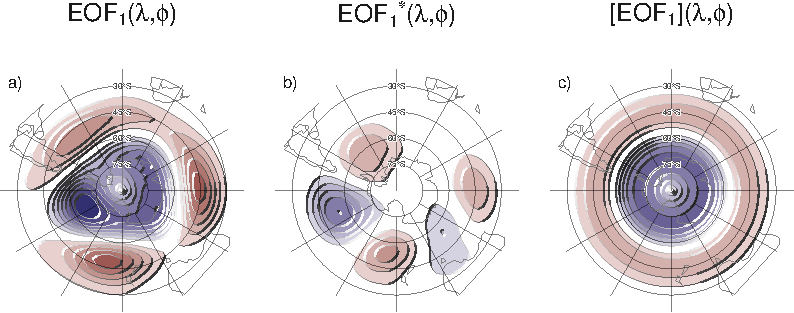
\includegraphics{method-1} \caption[Spatial patterns of the first EOF of 700 hPa geopotential height for 1979 -– 2018 period]{Spatial patterns of the first EOF of 700 hPa geopotential height for 1979 -– 2018 period. (a) Full field, (b) zonally asymmetric component and (c) zonally symmetric component. Arbitrary units.}\label{fig:method}
\end{figure*}

Our method assumes linearity in the asymmetric component of the SAM. That means we assume that zonal symmetries associated with positive SAM are almost opposite and of the same magnitude to the ones associated with negative SAM. \citet{fogt2012}'s composites (their Figure 4) suggest that this might not be entirely valid, although we argue that much of that apparent non-linearity is due to the heterogenous nature of the selected years for constructing the composites. Using our data (from 1979 to 2018), seasonal composites of zonal anomalies of geopotential height for SAM+ (Full SAM index greater than 1 standard deviation) and SAM- (less than minus 1 standard deviation) show relatively high pattern correlations for all seasons and are visually very linear both for the troposphere (represented by the 700 hPa level) and the stratosphere (represented by the 50 hPa level) (Figures A3 and A4). Therefore, we believe that our method is a reasonable approximation of the phenomenon.

By computing a single EOF pattern using data for all months we are assuming that the zonal anomalies of the SAM are the same in all seasons -- December to February (DJF), March to May (MAM), June to August (JJA) and September to November (SON). Geopotential zonal anomalies computed by projecting the first EOF of each season independently are very similar to each other in the troposphere (Figure A5, row 1) and show pattern correlations between 0.65 (DJF with JJA) and 0.9 (MAM with SON). In the stratosphere (Figure A5, row 2), patterns are similar for all trimesters except DJF, when the wave-1 zonal anomalies are rotated 90\degree~in comparison with the rest of the year. Pattern correlations in the stratosphere are between -0.24 (DJF with SON) and 0.95 (MAM with JJA). Based on this, we believe that our initial assumption is not unreasonable throught most of the year with the exception of DJF in the stratosphere.

Finally, we assume that the zonally asymmetric pattern is stationary in time. \citet{silvestri2009} suggest that this might not be the case between 1958 and 2004 but the period we analyse is much shorter (1979 -- 2018) so it's unlikely that we could observe significant changes. Moreover, zonal asymmetry of the spatial patterns for the two halves of the period (1979 to 1998 and 1999 to 2018) show no systematic change neither in the stratosphere nor in the troposphere (Figure A6).

\subsubsection{Regressions}

We perform linear regressions to quantify the association between the SAM indices and other variables. Since the Asymmetric and Symmetric SAM indices are significantly correlated with each other, to capture the variability explained uniquely by each index we use one multiple linear regression instead of two simple linear regressions. To obtain the linear coefficients of a variable \(X\) (geopotential, temperature, precipitation, etc\ldots{}) with the Asymmetric SAM (\(SAM_a\)) and Symmetric SAM (\(SAM_s\)) we fit the equation

\[
X(\lambda, \phi, t) = \alpha(\lambda, \phi) SAM_a + \beta(\lambda, \phi) SAM_s + X_0(\lambda, \phi) +  \epsilon(\lambda, \phi, t)
\]

where \(\lambda\) and \(\phi\) are the longitude and latitude, \(t\) is the time, \(\alpha\) and \(\beta\) are the linear regression coefficients, \(X_0\) and \(\epsilon\) are the constant and error terms. From this equation, \(\alpha\) represents the (linear) association of \(X\) with the variability of the Asymmetric SAM that is not explained by the variability of the Symmetric SAM; i.e.~it is proportional to the partial correlation of \(X\) and the Asymmetric SAM, controlling for the effect of the Symmetric SAM and vice versa for \(\beta\). When performing a separate regression for each trimester (DJF, MAM, JJA, SON), we average the relevant variables seasonally for each year and trimester before computing the regression.

At 2.5\degree by 2.5\degree resolution, a single regression field is composed of thousands of regressions. In such case, using p-values to test for significance leads to misleading results \citep{walker1914, katz1991}. While there are multiple proposed solutions in the literature, \citet{wilks2016} suggests that adjusting p-values by controlling for the False Discovery Rate \citep{benjamini1995} is a simple and effective method to ameliorate this issue. Therefore, p-values showed in regression fields are all adjusted following \citet{benjamini1995}.

We computed linear trends by Ordinary Least Squares and the 95\% confidence interval assuming a t-distribution of the appropriate residual degrees of freedom. To compute the amplitude of the zonal waves we computed the Fourier transform of the spatial field at each latitude circle.

We computed density probability estimates using a gaussian kernel of optimal bindwidth according to \citet{sheather1991}.

\subsubsection{Computation procedures}

We performed all analysis in this paper using the R programming language \citep{rcoreteam2020}, using the data.table package \citep{dowle2020} and the metR package \citep{campitelli2020}. All graphics are made using ggplot2 \citep{wickham2009}. We downloaded data from ranalysis using the ecmwfr package \citep{hufkens2020} and indices of the ENSO with the rsoi package \citep{albers2020}. The paper was rendered using knitr and rmarkdown \citep{xie2015, allaire2019}.

\hypertarget{results}{%
\section{Results}\label{results}}

\hypertarget{temporal}{%
\subsection{Temporal evolution}\label{temporal}}

\begin{figure*}
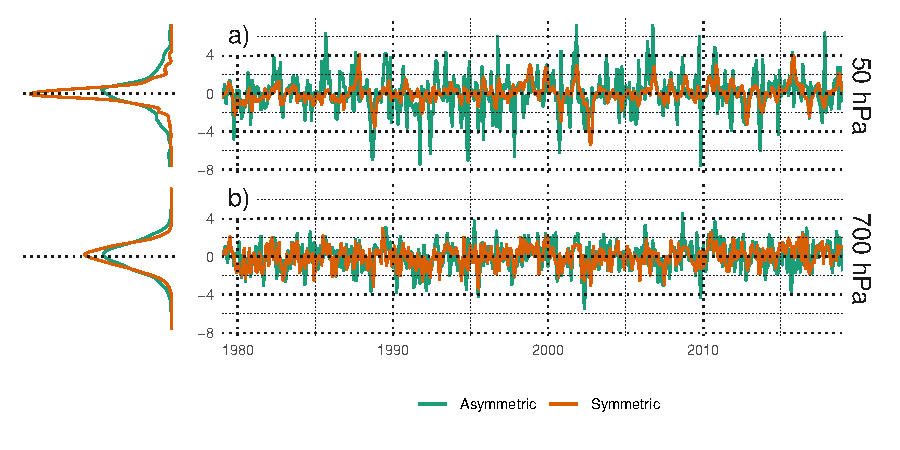
\includegraphics{asymsam-timeseries-1} \caption[Time series for the Asymmetric SAM and Symmetric SAM indices at (a) 50 hPa and (b) 700 hPa]{Time series for the Asymmetric SAM and Symmetric SAM indices at (a) 50 hPa and (b) 700 hPa. To the right, probability density estimate of each index. Series are standarised by the standard deviation of the Full SAM at each level.}\label{fig:asymsam-timeseries}
\end{figure*}

We first asses the temporal evolution of the Asymmetric SAM and Symmetric SAM. Figure \ref{fig:asymsam-timeseries} shows the corresponding time series for 700 hPa and 50 hPa and their corresponding density estimates. We selected these two levels as representative of the tropospheric and stratospheric variability respectively. As will be shown later, both indices are highly coherent within each atmospheric layer, therefore is reasonable to take one level as representative of each layer.

Month-to-month variability is evident for both indices, with noisy variations in the low frequency. At first glance the series can be distinguished by their distributions. Compared to the tropospheric indices, the stratospheric indices are much more long-tailed; that is, extreme values (both negative and positive) abound. The Asymmetric SAM series have both more variability in the higher frequencies than the Symmetric SAM series.

The stratospheric Symmetric SAM varies strongly with a two-year period, which can be seen by spectral analysis (Figure A2). This might suggests a link between stratospheric SAM variability and the Quasi-Biennial Oscillation \citep{baldwin2001b}. There is a local peak at 2 years in the periodogram of the tropospheric Symmetric SAM also, although it's not statistically significant. In the troposphere the most significant peak of variability is found in the Asymmetric index at around 3.6 months.

From Figure \ref{fig:asymsam-timeseries} we can see that the Asymmetric SAM and Symmetric SAM time series appear to be correlated. Moreover, looking at the extremes in the stratosphere, the Symmetric SAM series appears to lag the Asymmetric SAM series (see, for example, the positive events on late 1987). We show these correlations, across all the levels of the reanalysis for zero and -1 lag (Asymmetric SAM index leading the Symmetric SAM index), in Figure \ref{fig:cor-lev}. Zero-lag correlations between the Asymmetric SAM and Symmetric SAM series are relatively constant throughout the troposphere, fluctuating between 0.39 and 0.45. One-month-lag correlations are similarly constant but significantly reduced to around 0.17. In the stratosphere, zero-lag correlations drop to a minimum of 0.21 at 20 hPa and then it increases again monotonically with height up to the uppermost level of the reanalysis (although results near the top of the models are to be interpreted with care). At the same time, one-month-lag correlations increase with height. As a consequence, stratospheric Asymmetric SAM index tend to precede corresponding Symmetric SAM index.

\begin{figure}
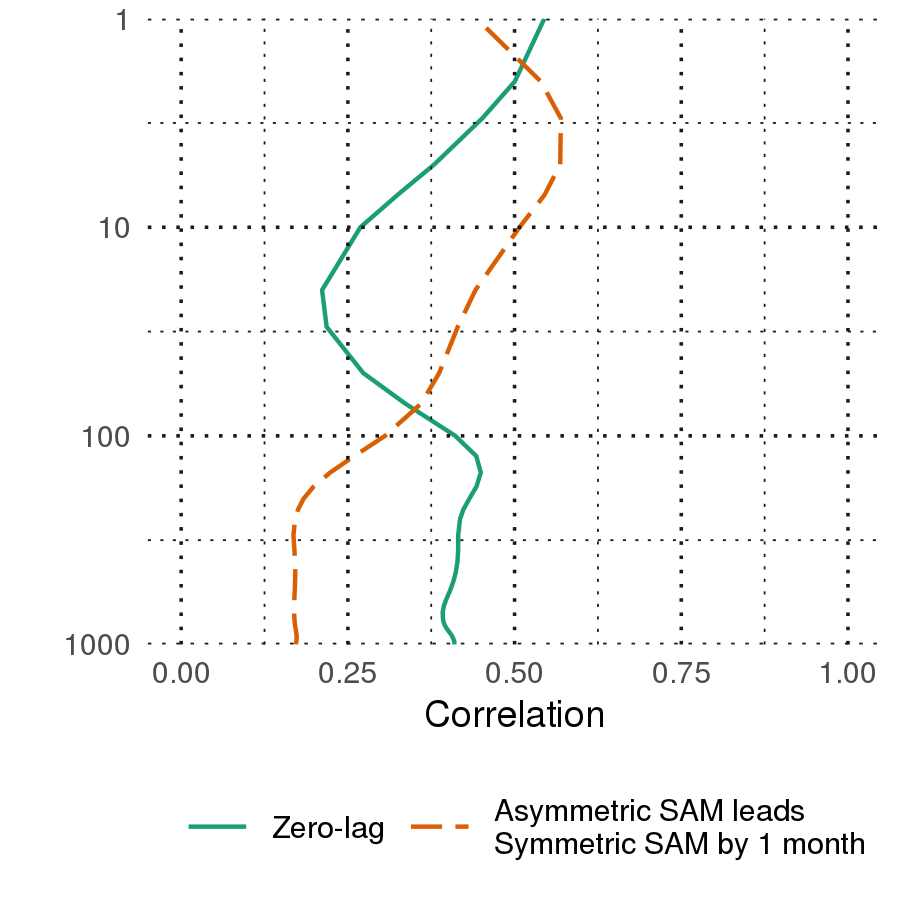
\includegraphics{cor-lev-1} \caption[Correlation between the Symmetric SAM and Asymmetric SAM index at each level for lag zero and lag -1 (Asymmetric SAM leads Symmetric SAM) for the 1979 -- 2018 period]{Correlation between the Symmetric SAM and Asymmetric SAM index at each level for lag zero and lag -1 (Asymmetric SAM leads Symmetric SAM) for the 1979 -- 2018 period.}\label{fig:cor-lev}
\end{figure}

\begin{figure*}
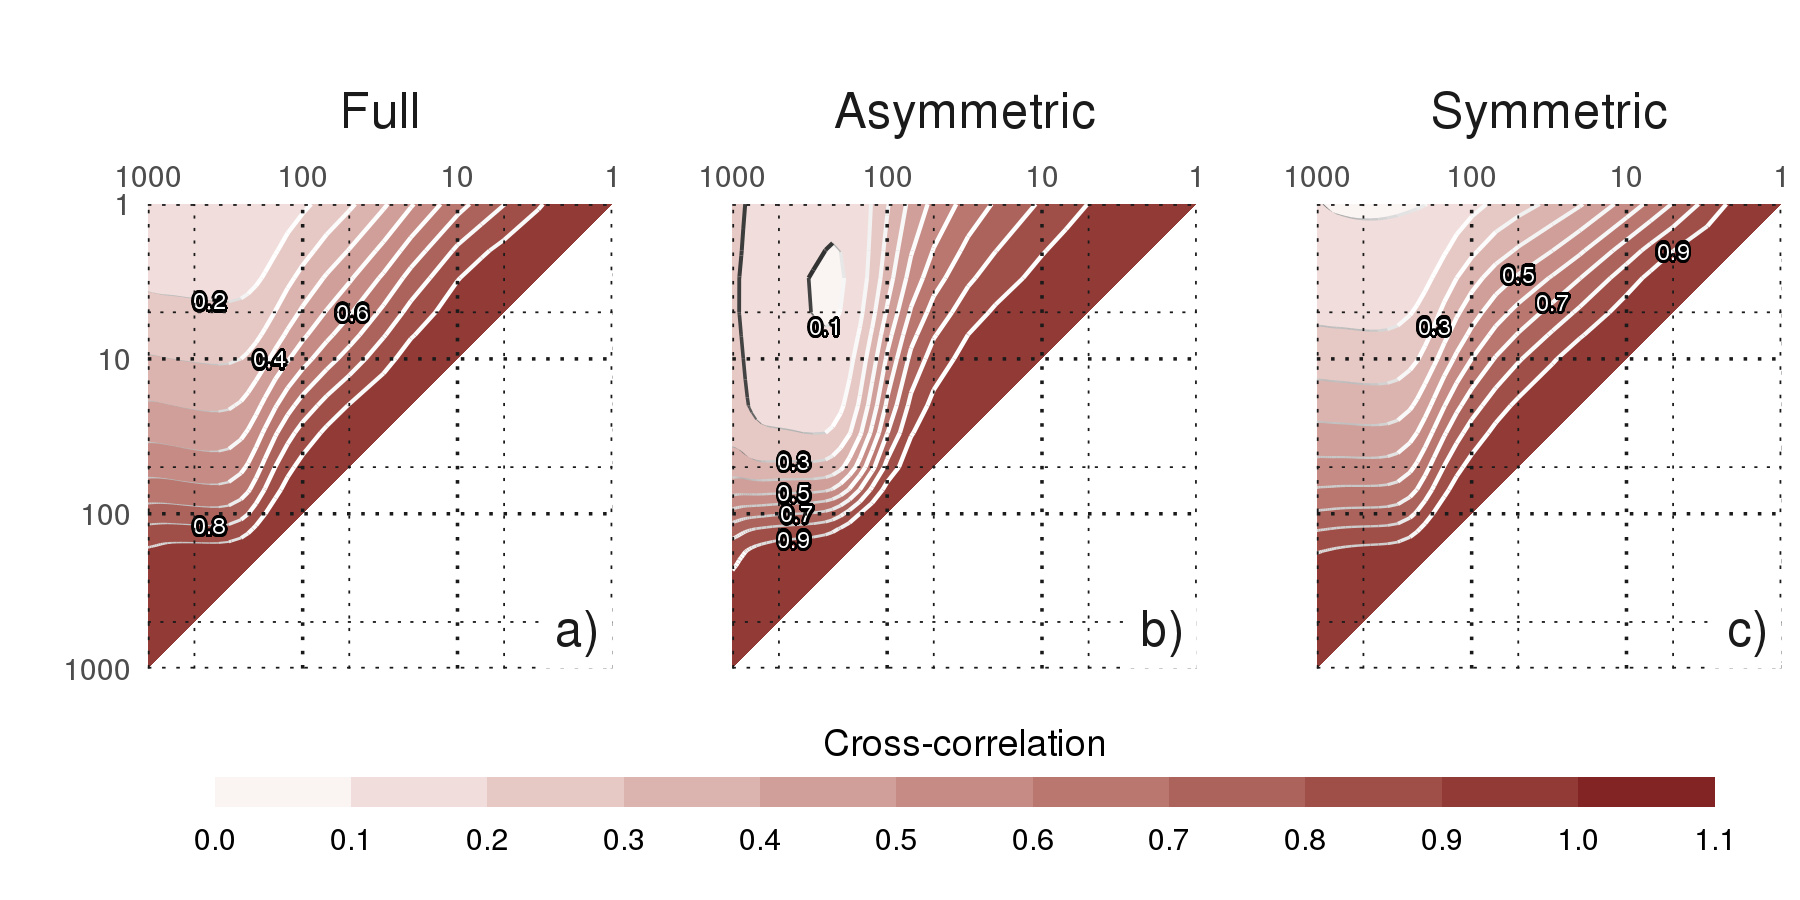
\includegraphics{cross-correlation-1} \caption[Cross correlation between levels of the (a) Full SAM, (b) Asymmetric SAM, and (c) Symmetric SAM for the 1979 -- 2018 period]{Cross correlation between levels of the (a) Full SAM, (b) Asymmetric SAM, and (c) Symmetric SAM for the 1979 -- 2018 period.}\label{fig:cross-correlation}
\end{figure*}

Figure \ref{fig:cross-correlation}a shows (zero-lag) cross-correlation across levels for the Full, Symmetric and Asymmetric SAM indices. For the Full SAM (panel a), high values below 100 hPa reflect the vertical (zero-lag) coherency throughout the troposphere. Above 100 hPa correlation between levels falls off more rapidly, indicating less coherent (zero-lag) variability. Therefore, there is a non negligible correlation between the troposphere and the lower-to-middle stratosphere. Examining panels b and c, we see that the Asymmetric and Symmetric SAM share the same high level of coherency in the troposphere but they differ in their stratospheric behaviour. Stratospheric coherency is stronger for the Asymmetric SAM than the Symmetric SAM. The stratospheric Symmetric SAM seems to connect more strongly to the troposphere than the Asymmetric SAM.

\begin{figure*}
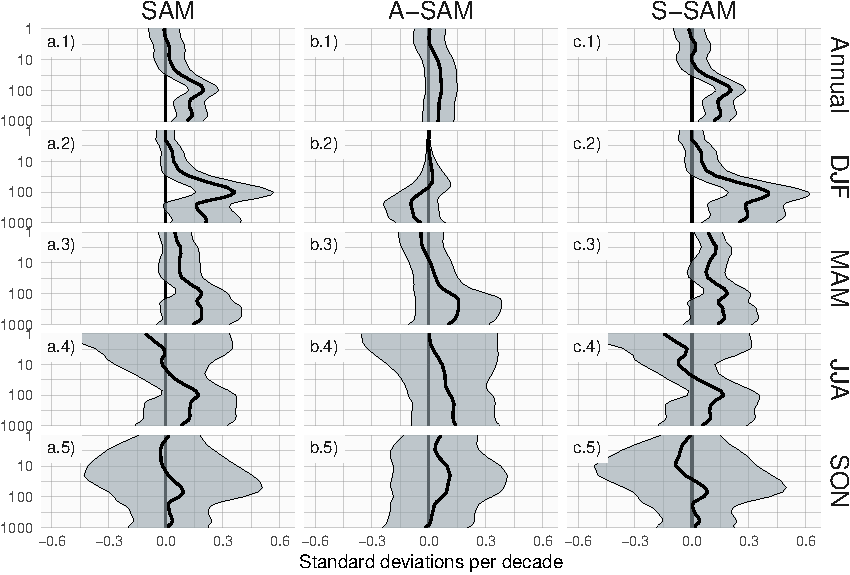
\includegraphics{trends-1} \caption[Decadal linear trends at each level for annual (row 1) and seasonal values (rows 2 to 5) for the period 1979 -- 2018 and for the (column a) Full SAM index, (column b) Asymmetric SAM index, and (column c) Symmetric SAM index]{Decadal linear trends at each level for annual (row 1) and seasonal values (rows 2 to 5) for the period 1979 -- 2018 and for the (column a) Full SAM index, (column b) Asymmetric SAM index, and (column c) Symmetric SAM index. Shading indicates the 95\% confidence interval from a t-distribution.}\label{fig:trends}
\end{figure*}

The linear trends for each of the indices (Full SAM, Symmetric SAM and Asymmetric SAM) were evaluated for the complete period 1979 -- 2018 at each level (Figure \ref{fig:trends}) for the whole year and separated by trimesters. The Full SAM index presents a statistically significant trend (panel a.1) that extends throughout the troposphere up to about 50 hPa and reaches its maximum value at 100 hPa. The seasonal trends (rest of column a) indicate that positive trends are present in Autumn and particularly in Summer, where the 100 hPa maximum is much more defined. In Winter and Spring, we detect no statistically significant trend. This is consistent with the results of previous studies, which find clear positive trends in Summer, weaker in Autumn and no trends in the other seasons \citep[e.g.][ and references therein]{fogt2020} using indices of the SAM based on surface or near-surface circulation.

By separating the SAM signal in its asymmetric and symmetric parts, we can not only see that these trends are almost entirely due to the symmetric component (column b vs.~column c), but in some cases the trends become more clear. In Summer, the Asymmetric SAM has a statistically non significant negative trend in the middle troposphere that obscures the trend in the Full SAM index; as a result, trends computed using only the Symmetric component are more clear (compare the shading region in panel a.2 and c.2). In Autumn, the Symmetric SAM reveals a statistically significant positive trend in the stratosphere that is not significant using the Full SAM index.

We stress that these are only linear trends during the whole period and the absence of a statistically significant signal should not be taken as evidence of no systematic change. In particular, going back to Figure \ref{fig:asymsam-timeseries}, we can see an evident change in the stratospheric Asymmetric component (red line in panel a) between the 90's, when we see a dominance of extreme negative values, and the 00's, when we see the inverse. This change is restricted to the Winter months: the linear trend for Winter starting in 1990 for the Asymmetric component at 50hPa is \(0.37 \pm 0.22\).

Figure \ref{fig:r-squared-trend} shows decadal trends for the explained variance of each index. There is no evidence of a significant trend in the stratosphere. In the troposphere, there is a positive trend for the Asymmetric SAM and not significant trend for the Symmetric SAM. This suggest that the SAM has become more asymmetric in the period from 1979 to 2018. However, the change is slight, around 1\% increased explained variance per decade.

\begin{figure}
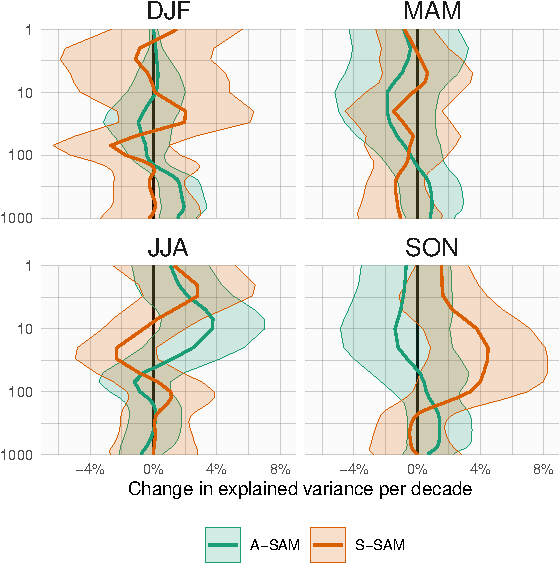
\includegraphics{r-squared-trend-1} \caption[Decadal trends of the variance explained by the Asymmetric and Symmetric SAM at each level for the period 1979 -- 2018]{Decadal trends of the variance explained by the Asymmetric and Symmetric SAM at each level for the period 1979 -- 2018. Shading indicates the 95\% confidence interval.}\label{fig:r-squared-trend}
\end{figure}

\hypertarget{spatial}{%
\subsection{Spatial patterns}\label{spatial}}

\begin{figure*}
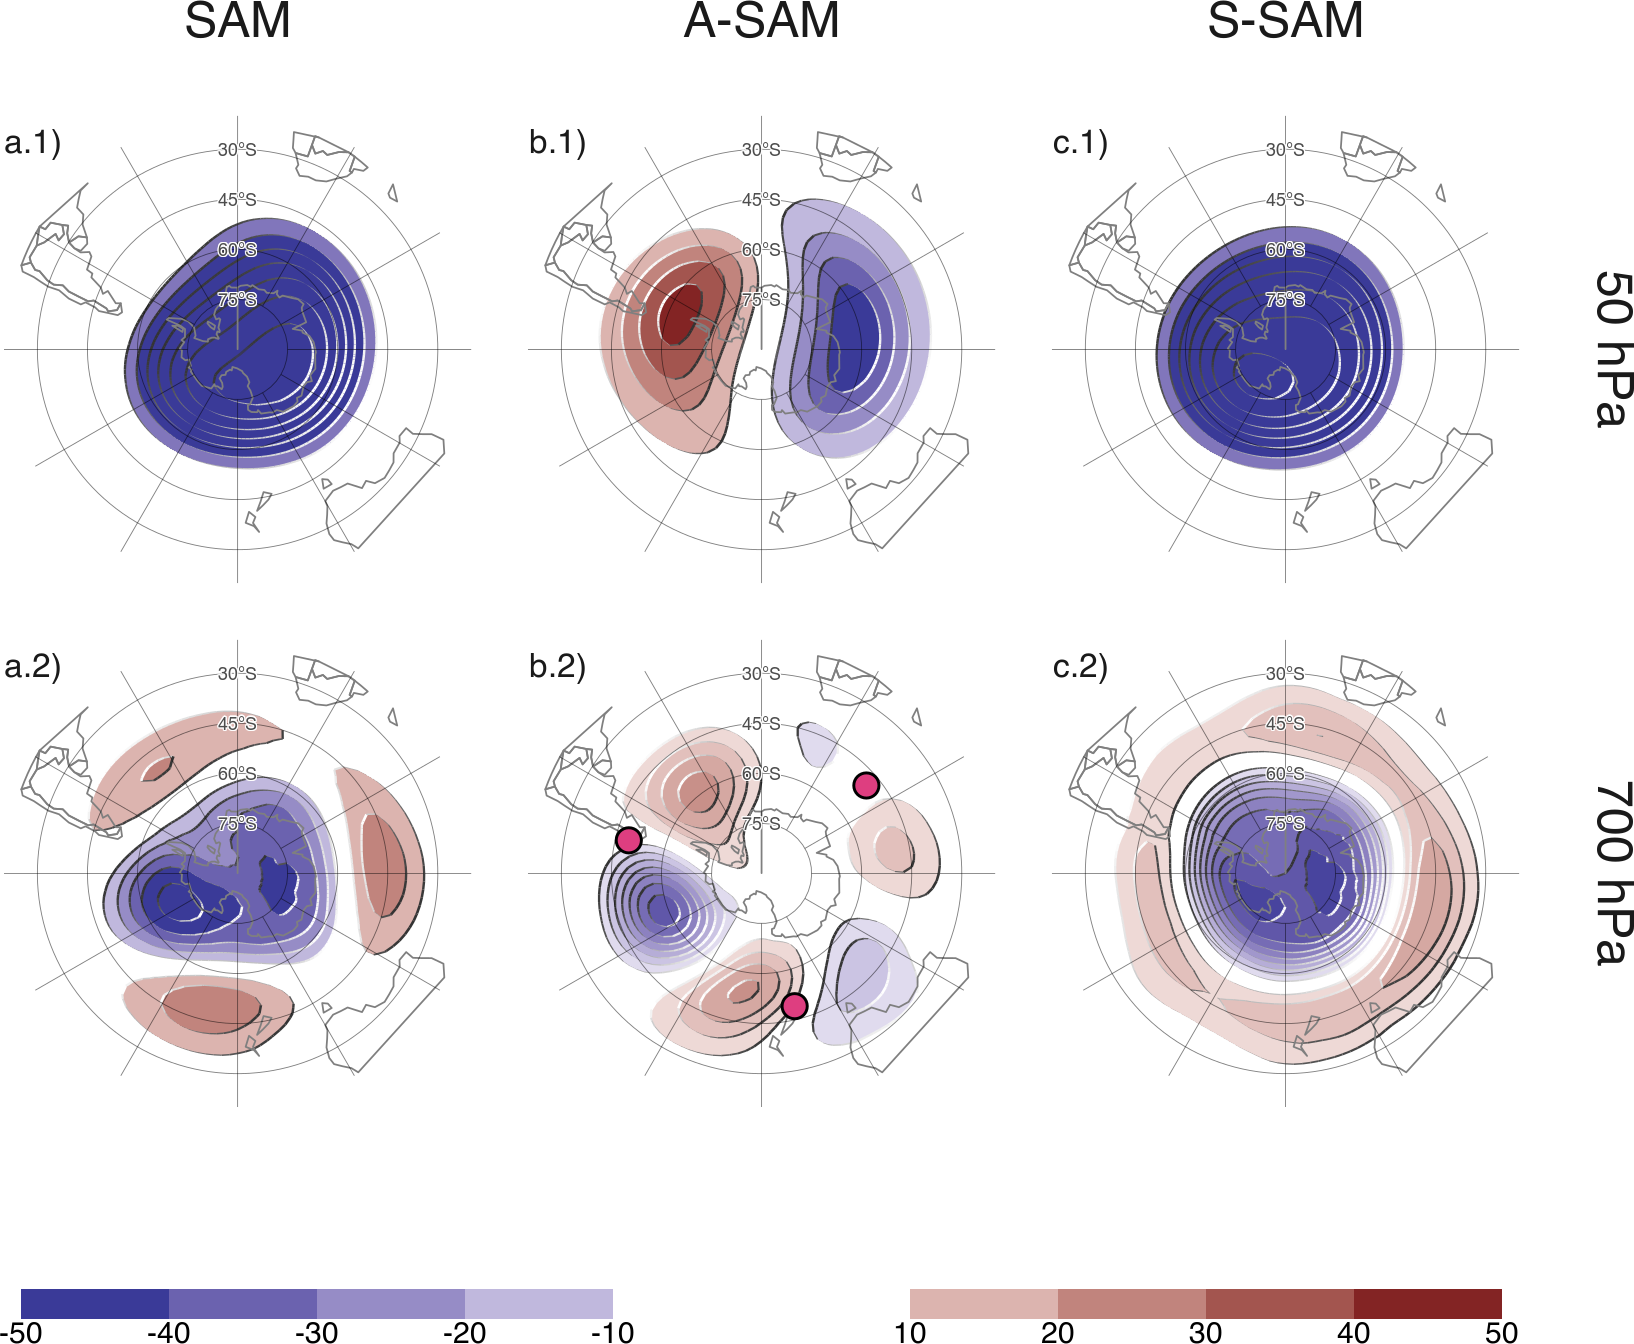
\includegraphics{2d-regr-1} \caption[Regression of geopotential height (meters) at (row 1) 50 hPa and (row 2) 700 hPa with the (column a) Full SAM, (column b) Asymmetric SAM, and (column c) Symmetric SAM for the 1979 -- 2018 period]{Regression of geopotential height (meters) at (row 1) 50 hPa and (row 2) 700 hPa with the (column a) Full SAM, (column b) Asymmetric SAM, and (column c) Symmetric SAM for the 1979 -- 2018 period. The regression patterns for Asymmetric and Symmetric SAM are the result of one multiple regression using both indices. Points marked on panel b.2 are the location of the reference points used by \cite{raphael2004} for their Zonal Wave 3 index. }\label{fig:2d-regr}
\end{figure*}

To show if, and to what extent, the Asymmetric and Symmetric SAM indices indeed capture the asymmetric and symmetric component of the SAM respectively, we computed the spatial regression of geopotential height anomalies on these indices and the Full SAM index for 700 hPa and 50 hPa levels. Figure \ref{fig:2d-regr} shows these regressions. Regression coefficients in column a are computed using the Full SAM. Regression coefficients in columns b and c are computed using multiple regression using the Asymmetric and Symmetric indices at the same time. Thus, they are to be interpreted as the patterns associated with each index, removing the variability (linearly) explained by the other index.

In the stratosphere, the spatial pattern associated with the Full SAM is more clearly dominated by a zonally symmetric, monopolar structure (panel a.1) which is, however, not perfectly centred in the South Pole. The monopole obtained by the regression pattern for Symmetric SAM (panel c.1) is much more symmetric and the shift from total symmetry is captured by the regression pattern of the Asymmetric SAM as a wave-1 with maximum anomalies above the Belinghausen Sea on the Western Hemisphere and and Davis Sea in the Eastern Hemisphere (panel b.1).

In the troposphere, panel a.2 shows the well known combination of zonally symmetrical annular mode with zonal asymmetries in the form of a wave-3 \citep{fogt2012}. The regression using the Asymmetric and Symmetric SAM indices successfully disentangle both structures. The Asymmetric SAM index gives rise to a cleaner zonal wave (panel b.2) and the Symmetric SAM index is associated with an annular mode, almost devoid of zonal asymmetries (panel c.2). The wave-3 pattern observed in panel b.2 is rotated by half a wavelength from the average position of the mean wave-3 pattern associated with \citet{raphael2004}'s ZW3 index, whose reference locations are marked with points in the figure. Thus, the tropospheric Asymmetric SAM index represents a zonal displacement in the position of the climatological wave-3 pattern.

\begin{figure*}
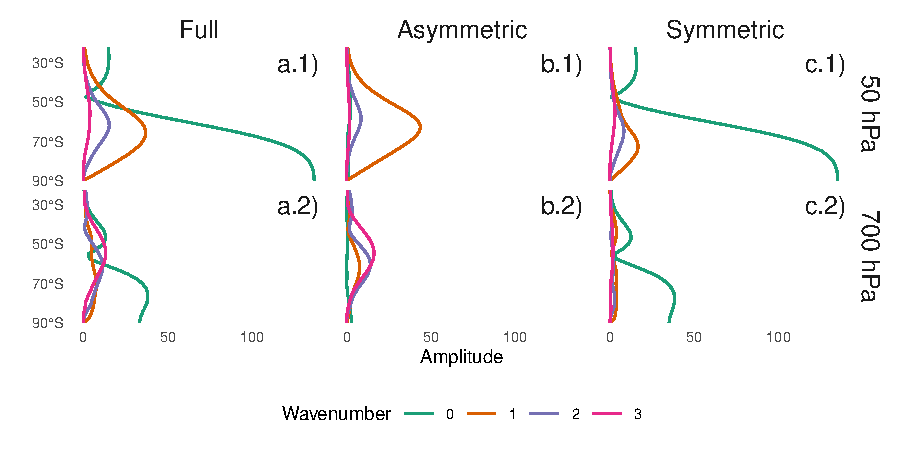
\includegraphics{wave-amplitude-1} \caption[Amplitude (meters) of zonal waves of the geopotential height regression patterns in Figure \\ref{fig:2d-regr} for zonal waves with wave-number 0, 1, 2, and 3, where wave-number 0 represents the amplitude of the zonal mean]{Amplitude (meters) of zonal waves of the geopotential height regression patterns in Figure \\ref{fig:2d-regr} for zonal waves with wave-number 0, 1, 2, and 3, where wave-number 0 represents the amplitude of the zonal mean.}\label{fig:wave-amplitude}
\end{figure*}

The amplitude of the first zonal wave numbers at each latitude at 50 hPa and 700 hPa is shown in Figure \ref{fig:wave-amplitude}, where wave number zero represents the amplitude of the zonal mean. Zonal wave amplitudes of the spatial pattern described by the Full SAM index (column a) are dominated by the zonal mean (wave-number 0) at both levels. However, zonal waves are important, particularly North of 50\degree S, with wave-number 1 clearly dominating at 50 hPa (panel a.1) and a more equal mix of waves at 700 hPa (panel a.2). Column b shows that the Asymmetric SAM is overwhelmingly dominated by wave 1 in the stratosphere (panel b.1), while in the troposphere it is composed of zonal waves 3 to 1 in decreasing level of importance (panel b.2) with negligible amplitude of the zonal mean. The Symmetric SAM, on the other hand, it's almost entirely composed of zonal mean at both levels (column c), with little to now contribution from zonal waves with wave-numbers 1 to 3.

We can see that the amplitude and latitudinal distribution zonal waves in the Asymmetric SAM on one hand, and the zonal mean in the Symmetric SAM on the other correspond almost exactly to the amplitude and latitudinal distribution in the Full SAM. This confirms the correct decomposition of the SAM in its symmetric and asymmetric components. Looking at panel b.2 from Figure \ref{fig:2d-regr}, it becomes apparent that zonal waves 1 and 2 modulate the amplitude of zonal wave 3, which -- as mentioned before -- is larger in the Western Hemisphere than in the Eastern Hemisphere.

\begin{figure}
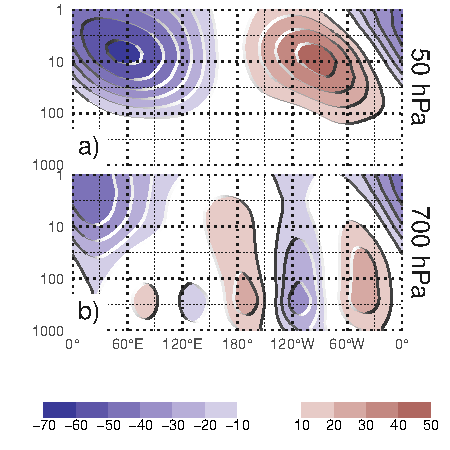
\includegraphics{vertical-regression-1} \caption[Regression between monthly geopotential height anomalies (meters) averaged betweeen 65\degree and 40\degree S and the Asymmetric SAM index (extracted from multiple regression including the Symmetric SAM)]{Regression between monthly geopotential height anomalies (meters) averaged betweeen 65\degree and 40\degree S and the Asymmetric SAM index (extracted from multiple regression including the Symmetric SAM). (a) With the Asymmetric SAM in 50 hPa and (b) in 700 hPa for the 1979 -- 2018 period.}\label{fig:vertical-regression}
\end{figure}

To analyse the vertical structure of the geopotential height anomalies associated with the asymmetric SAM index, we show a vertical cross section of regressions of mean geopotential height between 65\degree S and 40\degree S for the 50 hPa Asymmetric SAM index (panel a) and for the 700 hPa Asymmetric SAM index (panel b) (Figure \ref{fig:vertical-regression}). The geopotential height anomalies associated with the stratospheric Asymmetric SAM (panel a) are clearly constrained to the stratosphere, which underscores the uncoupling between the stratospheric and tropospheric Asymmetric SAM. The vertical structure of this signal tilts about 60\degree to the West between 100 hPa and 1 hPa, suggesting baroclinic processes. Interestingly, the signal in the stratosphere maximises near 10 hPa despite using the 50 hPa index for the regression.

The tropospheric Asymmetric SAM (panel b) has significant signals that extend upwards to the uppermost levels of the reanalysis. In the troposphere, the wave-3 structure is equivalent barotropic with maximum amplitude at roughly 250 hPa. The anomalies are much more intense in the Western hemisphere, where they extent into the stratosphere. In the Eastern hemisphere the wave-3 signal is weaker and confined to the troposphere while negative anomalies dominate in the stratosphere. So, while the tropospheric Asymmetric SAM index is associated with stratospheric geopotential anomalies, these do not project strongly onto the stratospheric Asymmetric SAM. The structures shown in panels a and b in Figure \ref{fig:vertical-regression} are robust to the choice of index level. For any stratospheric (above 100 hPa) index, the resulting anomalies are very similar to the wave-1 structure with maximum near 10 hPa in panel a. Conversely, for any tropospheric (below 100 hPa) index, the result is very similar to panel b. The patterns mainly change in amplitude (not shown).

The wave-3 pattern from Figure \ref{fig:2d-regr} panel b.2 is very similar to the Pacific-South American Pattern \citep{mo1987, kidson1988} which is a teleconnection pattern associated with the ENSO \citep{karoly1989}. Indeed, \citet{fogt2011} showed that there is a significant relationship between the SAM and the ENSO. The correlation between the Full SAM and the ENSO as measured by the Oceanic Niño Index \citep[ONI,][]{bamston1997} is -0.16 (p-value = \ensuremath{2.8\times 10^{-4}}). Consistent with \citet{fan2007}, we show that this relationship is captured entirely by the Asymmetric SAM, as this index has a partial correlation of -0.26 (p-value = \ensuremath{6.3\times 10^{-9}}) with the ONI controlling for the effect of the Symmetric SAM, whereas the Symmetric SAM's partial correlation with the ONI is essentially null (0.019; p-value = 0.67). We performed the same analysis using the Multivariate ENSO Index \citep{wolter2011} and the Southern Oscillation Index \citep{ropelewski1987} to conclude that these results do not depend on the ENSO index used.

\hypertarget{impacts}{%
\subsection{Surface Impacts}\label{impacts}}

\begin{figure*}
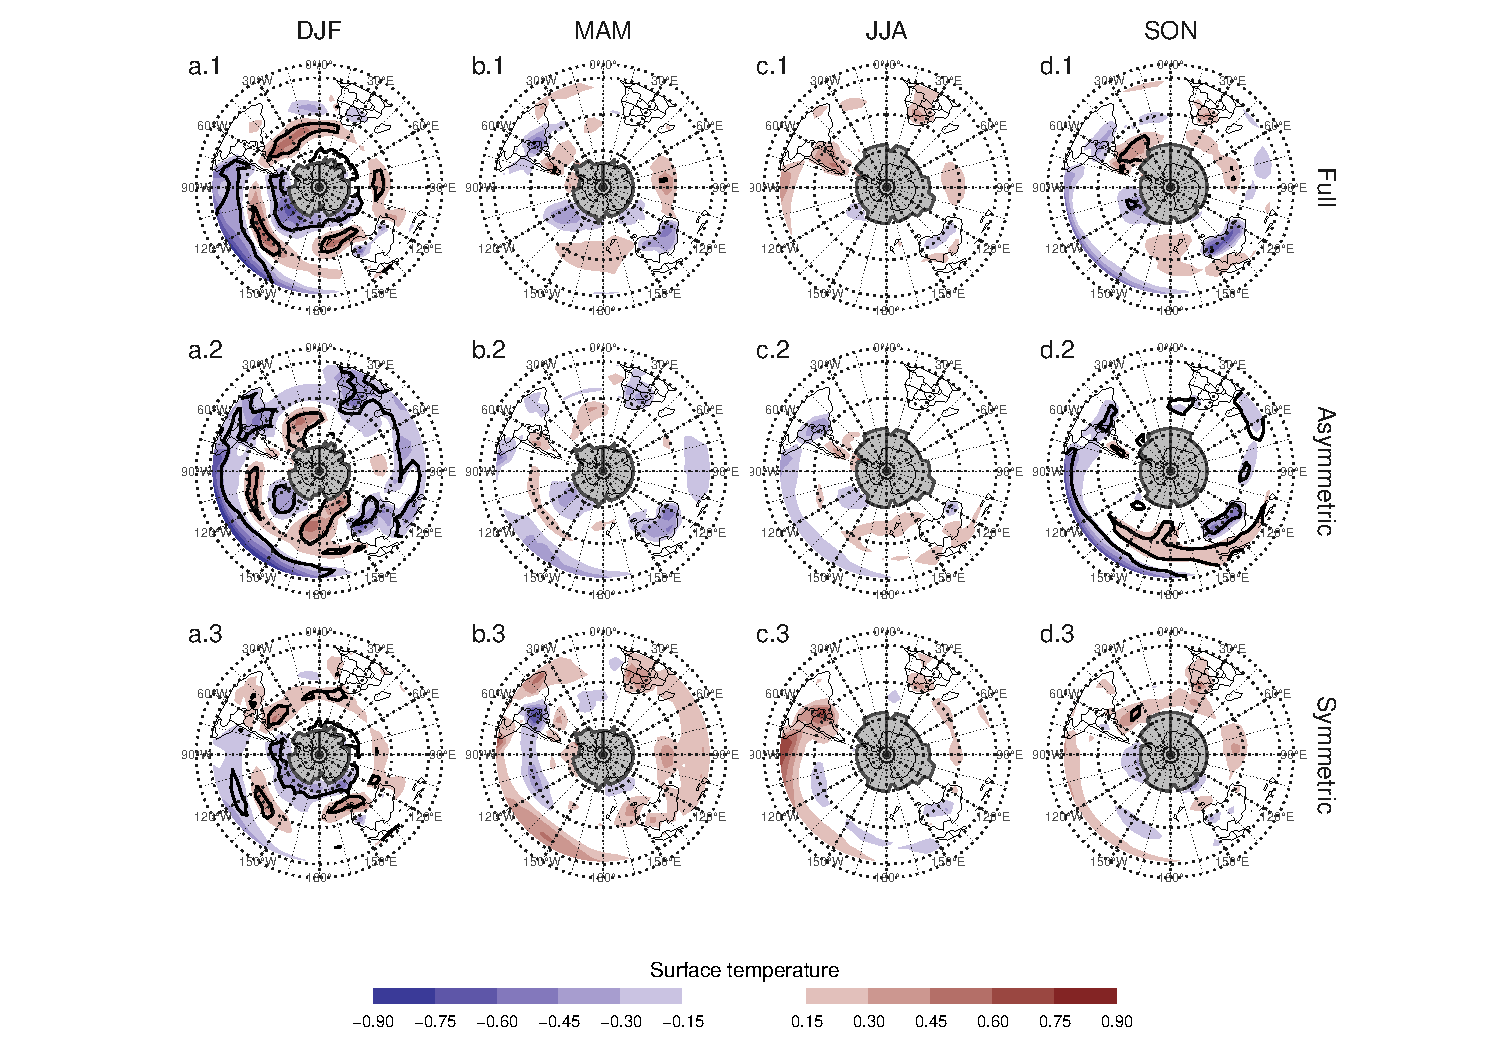
\includegraphics{regr-air-season-1} \caption[Regression of seasonal mean surface temperature (Kelvin) with Asymmetric SAM and Symmetric SAM for the 1979 -- 2018 period]{Regression of seasonal mean surface temperature (Kelvin) with Asymmetric SAM and Symmetric SAM for the 1979 -- 2018 period. Black contours indicate areas with p-value smaller than 0.05 controlling for False Detection Rate. Gray areas in Antarctica are areas with have more than 15\% of missing data.}\label{fig:regr-air-season}
\end{figure*}

To see if there are different surface impacts associated with the asymmetric and symmetric SAM circulation we regress surface temperature and precipitation onto each of the three SAM indices at 700 hPa. As shown in previous sections, the three indices are highly coherent in the troposphere, so we select this level to represent the tropospheric circulation for consistency with previous studies.

Figure \ref{fig:regr-air-season} shows regression coefficients of each index at 700 hPa with surface temperature for each trimester. In Summer, positive values of the Full SAM index (panel a.1) are associated with negative temperature anomalies near Antarctica which are surrounded by a ring of positive anomalies. The ring is not zonally symmetric, as there are four clear local maximums around 30\degree W, 120\degree W, 150\degree E and 90\degree E. In the tropics, there are negative anomalies in the equatorial Pacific, consistent with the negative correlation between SAM and ENSO. Panels b.1 and c.1 show temperature anomalies associated with positive values of the Asymmetric and Symmetric SAM, respectively. Both the local maximums in the ring and the anomalies in the Pacific regions are present mostly on the Asymmetric SAM regression map, while temperature patterns linked to positive Symmetric SAM show a more zonally consistent ring and less relation to the tropics. Noticeable, temperature anomalies in the Indian ocean, South Africa and Australia are strongly related to Asymmetric SAM. This signal is not present in the regression pattern with the Full SAM. Spring (row 4) features similar patterns but of smaller magnitude, with less regions where regressed anomalies have statistical significance.

In Autumn and Winter (rows 2 and 3) the positive ring is only present through its local maximums in the regression with the Full SAM. There are also negative anomalies in Southern Australia, and positive anomalies over New Zealand and Southern South America. These patterns are not significant in the sense that there are no areas with p-values below 0.05 when controlling for FDR following \citet{wilks2016}. However, repeating this analysis with 2-meter temperature from ERA5 resulted in similar patterns that were statistically significant (not shown). Moreover, similar features were observed in station measurements by \citet{jones2019}, although using data from 1957 to 2016.

The pattern of negative anomalies in the pole surrounded by positive anomalies roughly seen in all seasons -- although with varying intensity and small-scale details -- translates to enhanced meridional temperature gradient maximised in the zero line, which is consistent with the intensification and poleward migration of the westerlies commonly linked to the SAM through thermal wind balance. It's then not surprising to see it more clearly in association with the Symmetric SAM (at least in Summer and Spring).

Figure \ref{fig:regr-air-season} column b can be partially compared with Figure 11 from \citet{fogt2012}. Although they used station data from 1958 to 2001, main features are reproduced here, such as the strong signal in New Zealand and Australia in Summer and Spring.

Regression of the SAM indices with seasonal mean precipitation and 700 hPa geopotential height are shown in Figures \ref{fig:pp-regr-oceania} and \ref{fig:pp-regr-america} for Australasia and South America respectively. South Africa is not shown because no significant signal was detected there.

\begin{figure*}
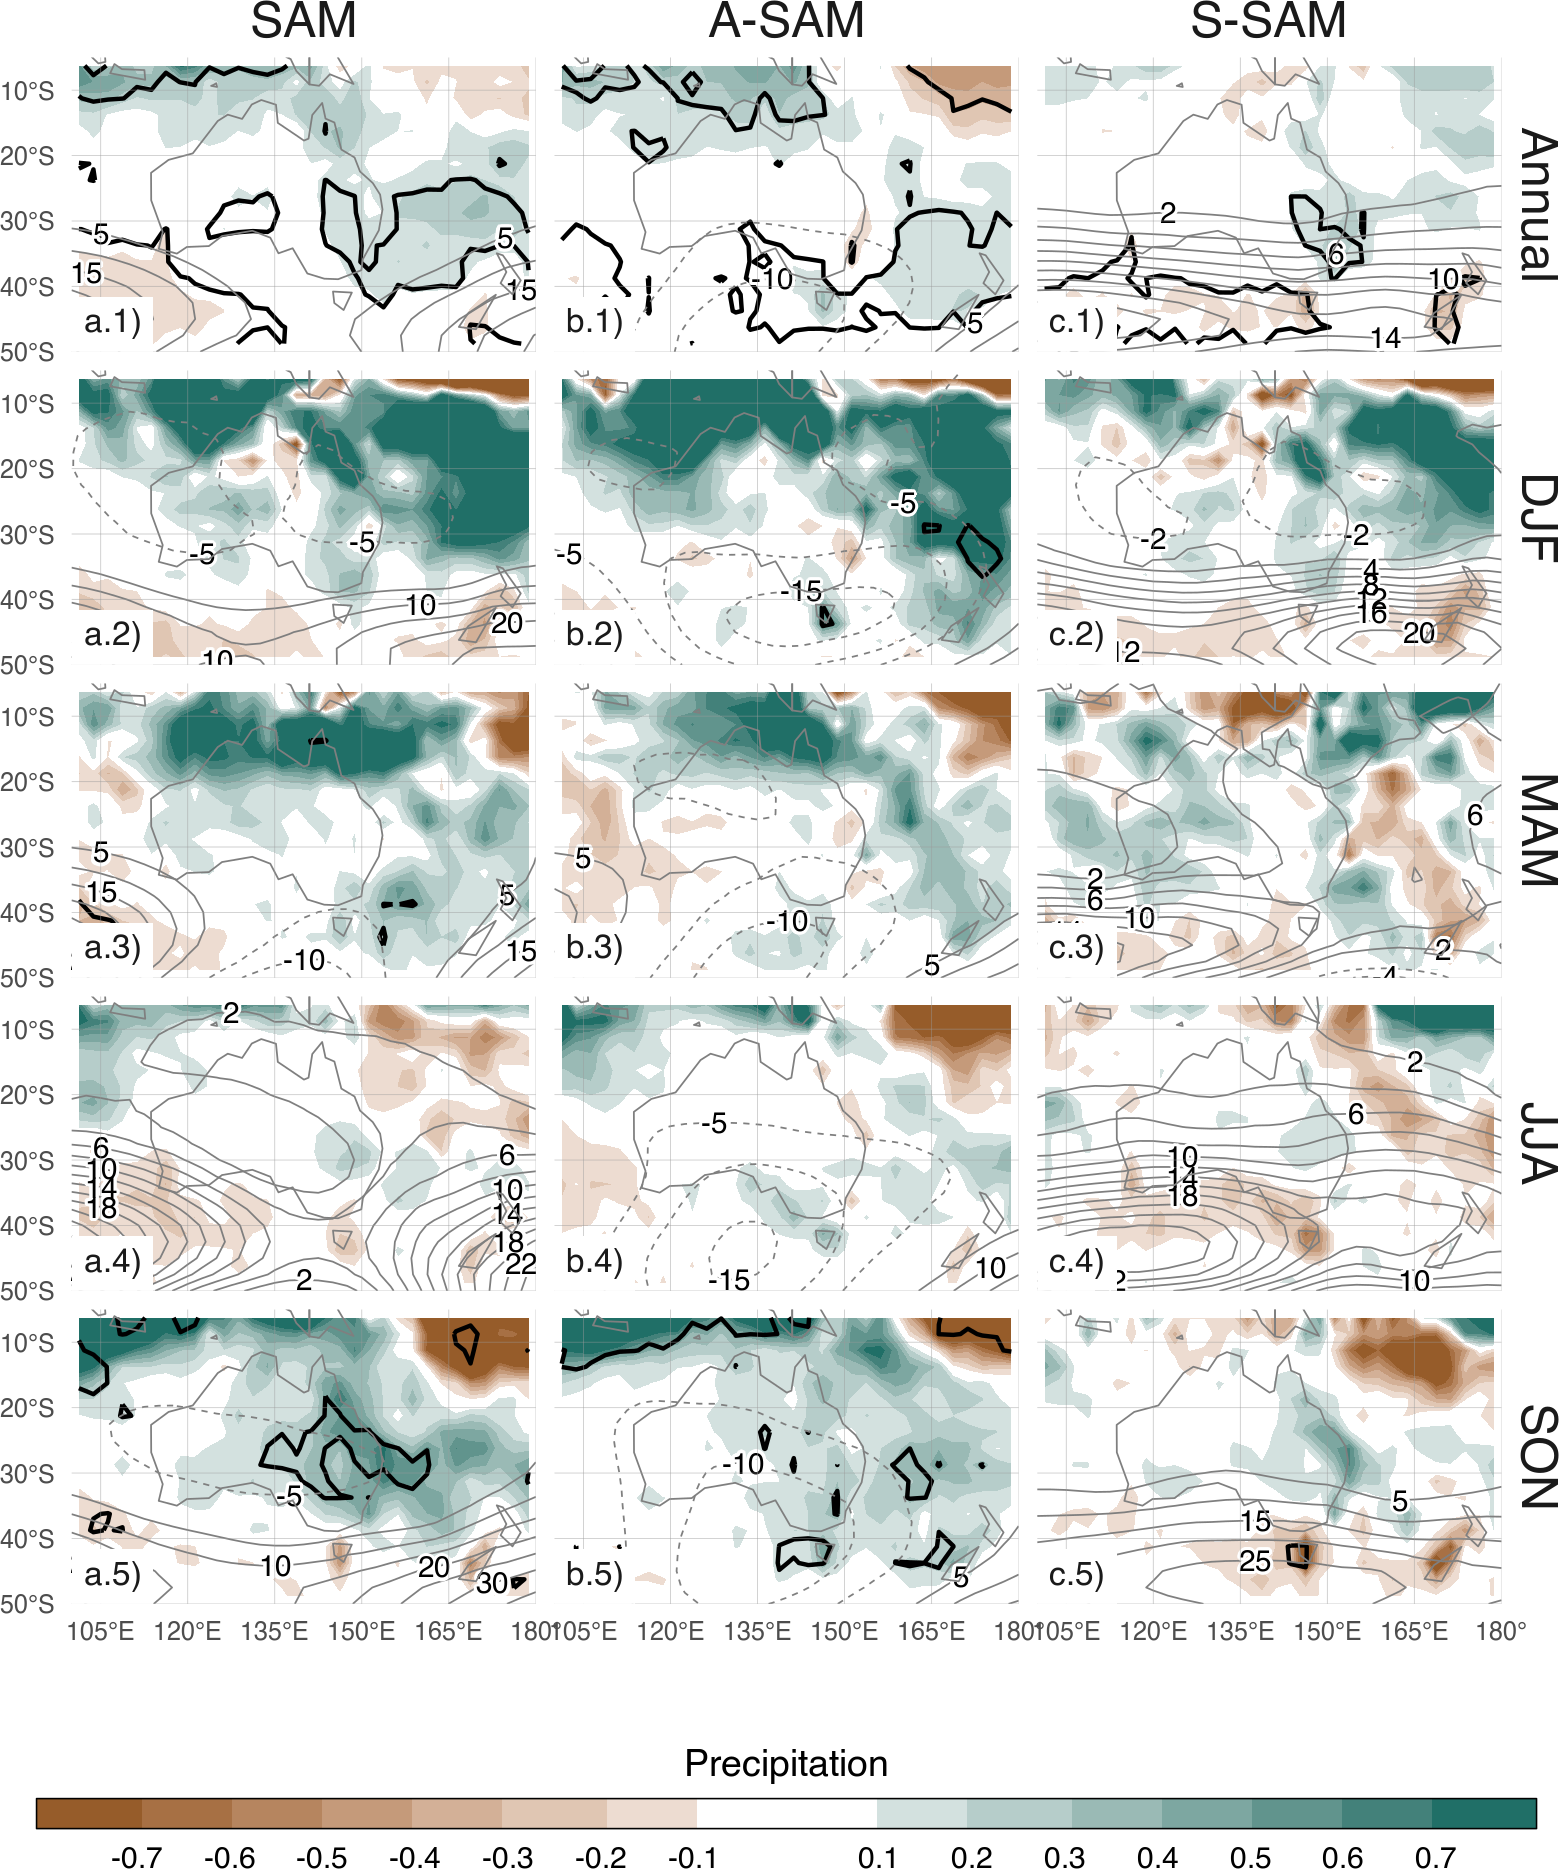
\includegraphics{pp-regr-oceania-1} \caption[Regression of (row 1) annual and (rows 2 to 5) seasonal mean precipitation anomalies (mm per day, shading) and 700 hPa geopotential height (thin lines, positive values as solid lines and negative values as dashed lines) with (column a) Full SAM, (column (b) Asymmetric SAM and (column c) Symmetric SAM for the 1979 -- 2018 period]{Regression of (row 1) annual and (rows 2 to 5) seasonal mean precipitation anomalies (mm per day, shading) and 700 hPa geopotential height (thin lines, positive values as solid lines and negative values as dashed lines) with (column a) Full SAM, (column (b) Asymmetric SAM and (column c) Symmetric SAM for the 1979 -- 2018 period. Thin lines are the Black contours indicate areas with p-value smaller than 0.05 controlling for False Detection Rate.}\label{fig:pp-regr-oceania}
\end{figure*}

In Australia, the annual regression shows that the Full SAM index is positively associated with precipitation in the Southeastern region (Figure \ref{fig:pp-regr-oceania} panel a.1), which reproduces the results from \citet{gillett2006}. The separation between Asymmetric and Symmetric SAM suggest that this positive anomaly is explained by the Symmetric SAM only in the East coast (panel c.1). Geopotential anomalies associated with this index (black contours) are indicative of easterly flow from the Tasman Sea, which could explain the positive anomalies in precipitation as found by \citet{hendon2007}. The Asymmetric SAM appears related to increased precipitation in the West coast of Southeastern Australia (panel b.2), which could similarly be explained by the anomalous westerly circulation transporting moist air to the continent from the Indian Ocean.

The seasonal-level regressions show statistically significant anomalies only in Spring, when positive Full SAM is associated with positive precipitation anomalies in Eastern Australia (panel a.5). In this trimester the Symmetric SAM seems to be associated with precipitation in a relatively reduced area of the East Coast (panel c.5) while the positive precipitation anomalies related with positive Asymmetric SAM affect all Eastern Australia (panel b.5).

In Summer, positive Full SAM index is associated with with positive precipitation anomalies in Western and Eastern Australia, particularly in the North East (panel a.2). The Eastern part being dominated by the relationship with the Symmetric SAM and the Western, by the Asymmetric SAM. In Autumn, the regression with Full SAM shows positive values in the North, similar to Summer, and a broad area of positive values in the North-East to South-West direction. This structure seems to be associated with the Symmetric SAM, while the Northern positive values are associated with the Asymmetric SAM. In Winter we see the same NE to SW aligned anomaly (although with much reduced amplitude) that is also present only in relation with the Symmetric SAM. None of these regression coefficients are statistically significant at the 95\% level. The Spring signal is broadly consistent with \citet{hendon2007}, but whereas \citet{hendon2007} also detected a strong signal in Summer, panel a.2 shows no statistically significant association (although the coefficients have the consistent sign).

\begin{figure*}
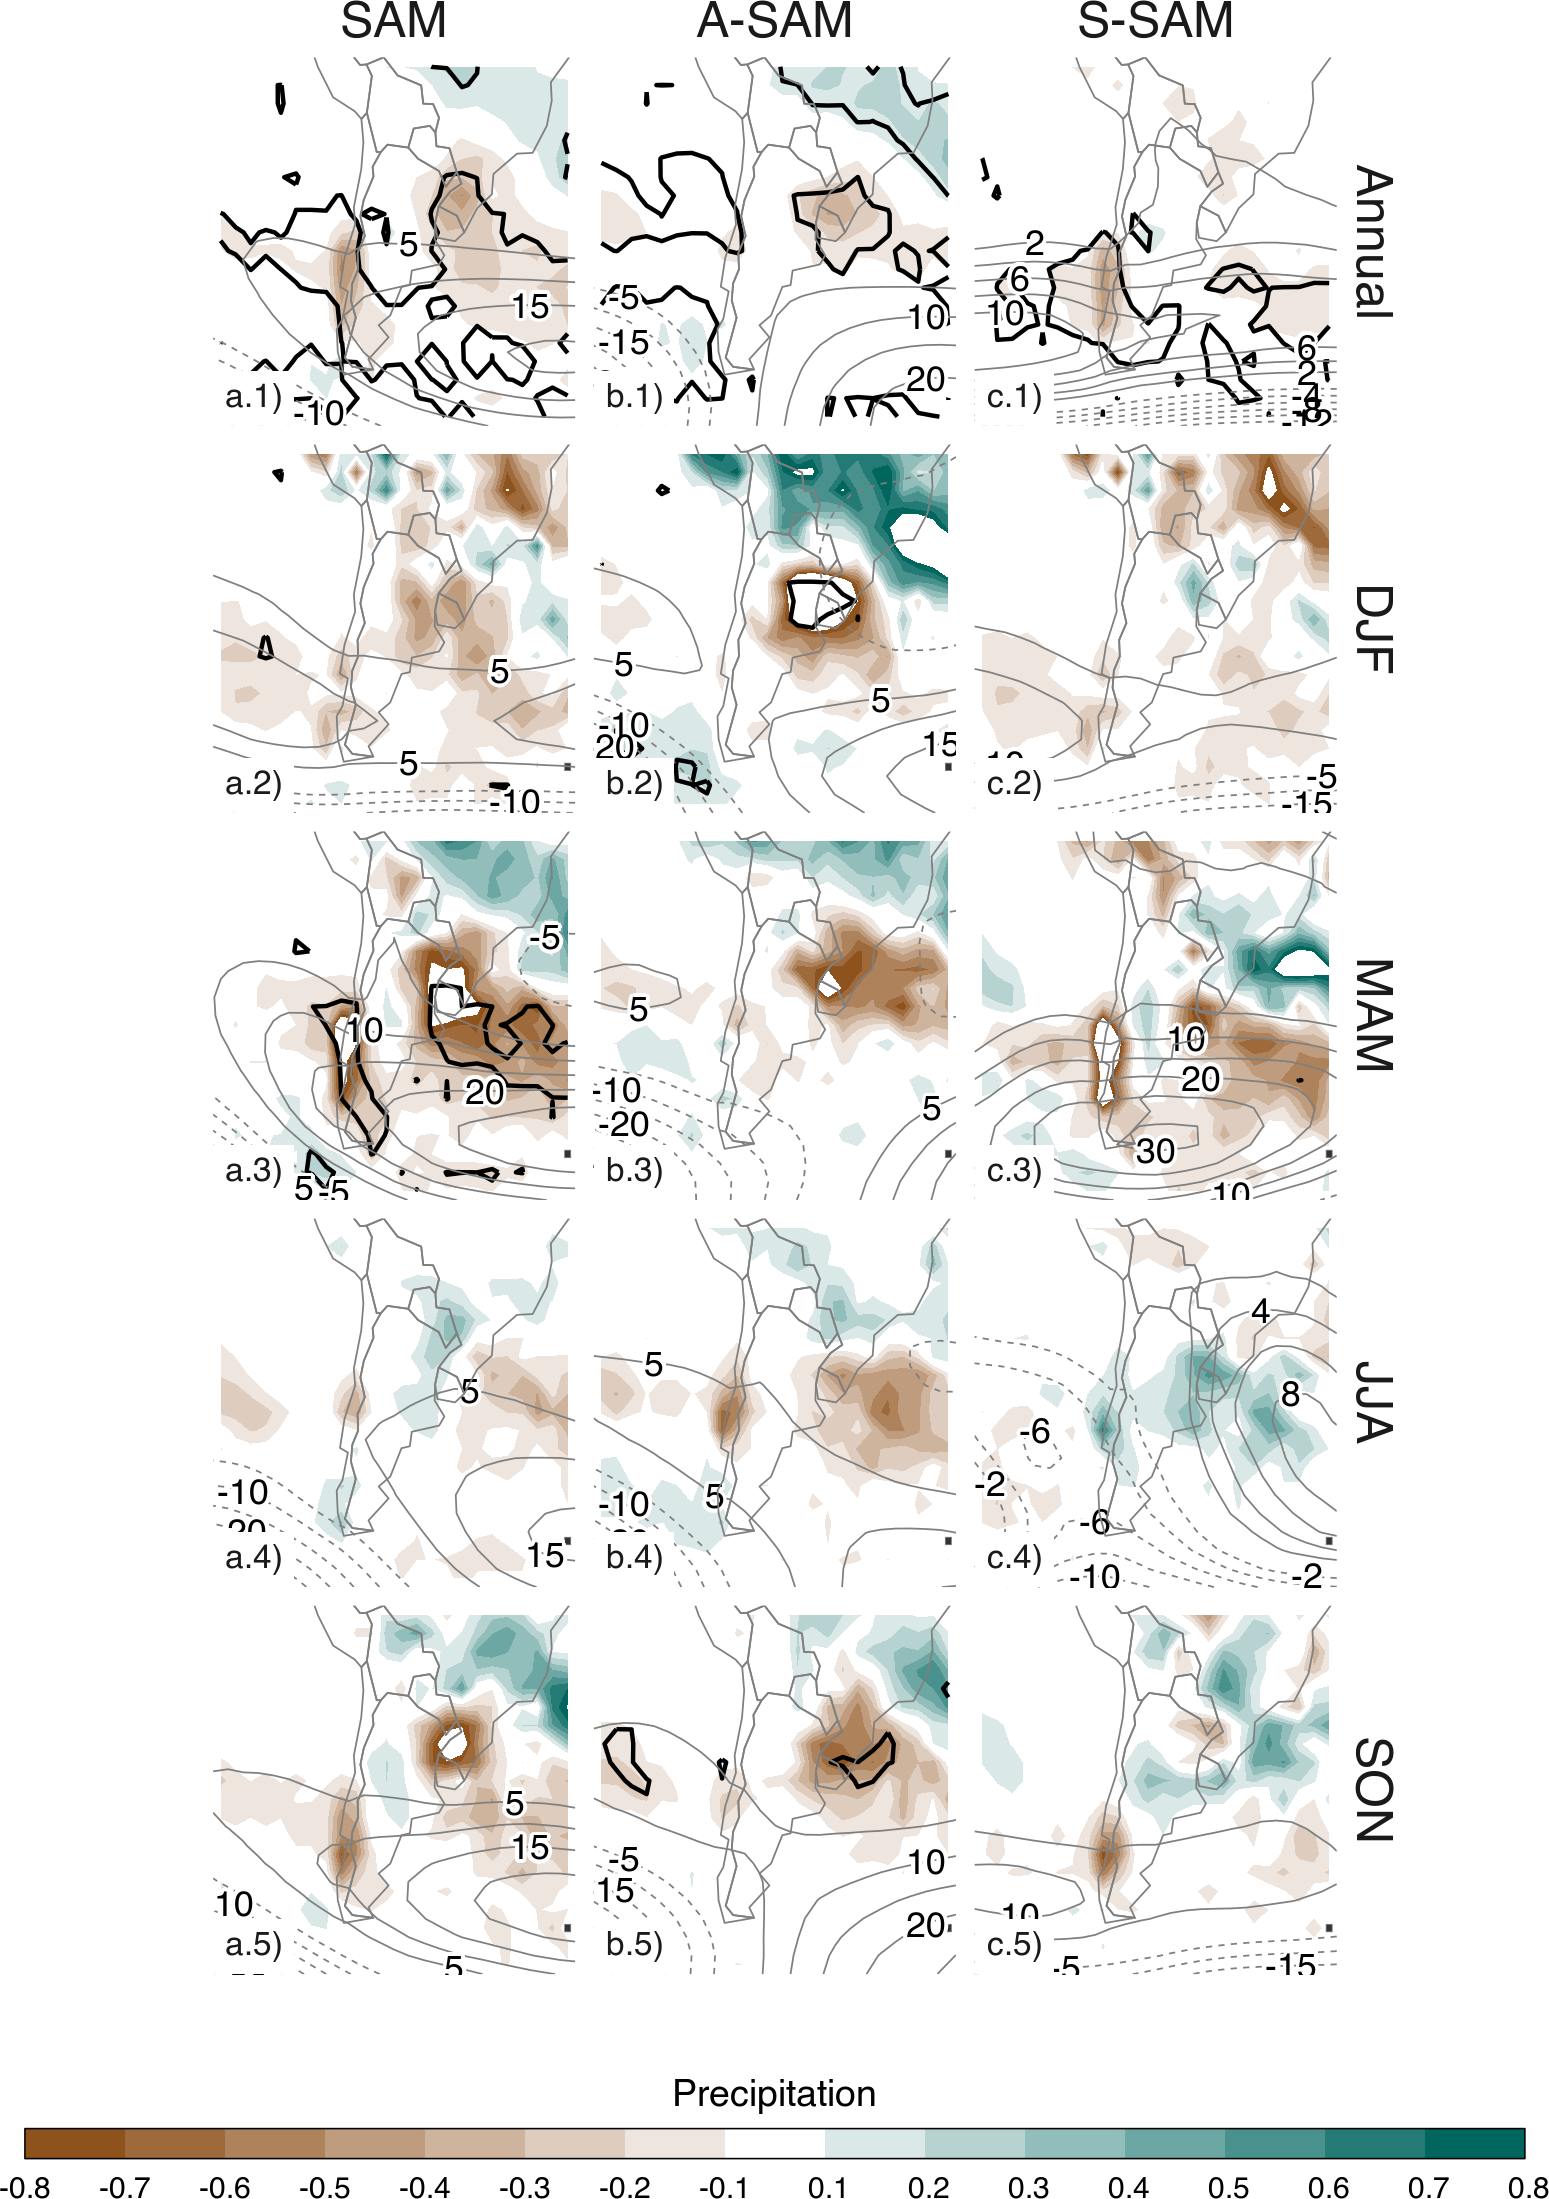
\includegraphics{pp-regr-america-1} \caption[Same as Figure \\ref{fig:pp-regr-oceania} but for South America]{Same as Figure \\ref{fig:pp-regr-oceania} but for South America.}\label{fig:pp-regr-america}
\end{figure*}

In South America (Figure \ref{fig:pp-regr-america}), the annual-level regression shows that positive SAM is associated with statistically significant precipitation decrease in Southeastern South America (SESA) and Southern Chile and non-significant increase in South Brazil, near the South Atlantic Convergence Zone (SACZ) (panel a.1). Panels b.1 and c.1 show a remarkably clean separation between the Asymmetric SAM -- associated with the Southeastern South American and Southern Brazilian signals -- and the Symmetric SAM -- associated with the signal in Southern Chile.

Except Winter, seasonal-level regressions mirror this same pattern. Even if not statistically significant, they all show negative values in Southeastern South America and Southern Chile along with positive values in Southern Brazil in relation with the Full SAM. The separation of these features between the Asymmetric SAM and Symmetric SAM regression maps is also rather consistent.

The anomalous circulation at 700 hPa associated with the Symmetric SAM (panel c.1) indicate anomalous Easterly flow over Southern Chile. This leads to reduced influx of moist air from the Pacific Ocean which, is the main source of precipitable water in that region \citep{garreaud2007}. On the other hand, the anomalous circulation associated with positive values of Asymmetric SAM (panel b.1) in the Atlantic is anticyclonic in the South and cyclonic in the North. This creates anomalous South-Easterly flow over Southeastern South America, which inhibits the flow of the Low Level Jet to the region \citep{silvestri2009, zamboni2010}. This same pattern was found to be associated with increased precipitation in Southern Brazil during South Atlantic Convergence Zone events \citep{rosso2018}. There is a small area of increased precipitation with SAM near central Argentina which is also present in the station-based analysis by \citet{gillett2006} and that is explained by the Asymmetric SAM.

\subsection{Conclusions}

In this study we characterise the temporal and spatial variability of the zonally symmetric and asymmetric structure of the SAM. By projecting monthly geopotential fields at each level with the corresponding asymmetric and symmetric pattern, we created two indices for representing the zonally asymmetric and symmetric contributions of the SAM respectively.

As expected, the Asymmetric SAM index correlates strongly with the Symmetric SAM index. In the troposphere, this correlation is maximum at zero lag, while in the stratosphere is maximised with the Asymmetric SAM leading the Symmetric SAM by one month. Since most indices of the SAM are calculated using surface or near-surface conditions, this result would suggest that they might not be sensitive to the most dramatic changes in SAM variability.

The two-year periodicity we found in the stratospheric Symmetric SAM might point to a link between the SAM and the Quasi Biennial Oscillation. There is evidence of influence between the QBO and the Northern Annular Mode \citep[e.g.][]{holton1980, watson2014, zhang2020}, so it's not unlikely that the SAM would be similarly connected. However establishing this link would require further research.

We observe a positive trend towards positive SAM in Summer and Autumn, As was documented by previous studies, such as \citet{fogt2020} (and references therein) for surface levels. We show that these trends are maximised at the 100 hPa level and are explained by the zonally symmetric component. We also find a statistically significant positive trend in the Symmetric component of the SAM in the stratosphere that is not apparent in the Full SAM index. In contrast to \citet{fogt2012} we find some evidence of the SAM becoming more zonally asymmetric, as there is a slight positive trend in the variance explained by the as the Asymmetric SAM explains an increasingly proportion of the total variance.

In the troposphere, the spatial patterns of geopotential associated with the Symmetric SAM are much closer to being truly annular than the patterns associated with the Full SAM index. The Asymmetric SAM, on the other hand, describes a wave-3 pattern with maximum amplitude in the Pacific region and whose phase is rotated a quarter wavelength from the mean zonal wave 3 described by \citet{raphael2004}'s index. This pattern extends in the troposphere but its maximum is located at 250 hPa, which also could suggest that surface-based indices are not optimum for capturing this variability.

This wave-3 pattern is similar to the Pacific-South American Pattern, which is a teleconnection pattern linked to ENSO variability. We found that the significant correlation that exists between the Full SAM index and the Oceanic Niño Index is captured entirely by the Asymmetric SAM index. This suggests that ENSO is linked to SAM exclusively through the variability in the latter's asymmetric component and thus, the Asymmetric SAM index could be a useful measure to further study that relationship.

Temperature anomalies associated with the Full SAM broadly show a pattern of negative anomalies at polar latitudes surrounded by positive anomalies, but with many deviations from symmetry. The Asymmetric SAM index explains a big portion of these deviations. In particular, the positive phase of the Asymmetric SAM is associated with colder temperatures over Southern Brazil, South Africa and Southern Australia, as well as the negative anomalies in the equatorial Pacific consistent with the ENSO-SAM relationship. These negative anomalies are particularly clear in the DJF and SON trimesters, which include the months in which the ENSO teleconnection is more active \citep{cazes-boezio2003, fogt2011, cai2020a}.

In Australia the Full SAM is associated with positive precipitation anomalies in South East and this is explained by the Symmetric SAM. However, the Asymmetric SAM is associated with a small area of positive precipitation anomalies in the Eastern Coast of West Australia, maybe due to advection of moist air from the Indian Ocean. In South America, precipitation anomalies associated with the Full SAM are negative both in Southern Chile and Southeastern South America, and positive in Southern Brazil. This features are cleanly separated between the Asymmetric and Symmetric components. The Symmetric SAM explains the negative anomalies in Southern Chile and the Asymmetric SAM, the negative-positive dipole between Southeastern South America and Southern Brazil. Individual seasons mostly follow this pattern.

\citet{silvestri2009} suggests that precipitation impacts linked to the SAM changed rather dramatically before and after 1980. In particular, the negative relationship with precipitation in South America was absent in some areas and switched sign in others in the earlier period. The correlation between ENSO and SAM is similarly non-stationary, also changing sign before the 1980s \citep{fogt2006, clem2013}. Seeing as both the ENSO-SAM relationship and most of the precipitation impacts in South America are captured by the Asymmetric SAM, the results presented here are most likely period-dependent.

By succesfully separating the zonally symmetric and zonally symmetric SAM signals, we show that the asymmetric component of the SAM has its unique variability, trends and impacts. This is particularly important in the context of a changing climate, as the impact on the SAM of ozone recovery is modeled as highly zonally symmetric, while the impact of increased concentration of greenhose gases has also a zonally asymmetric component \citep{arblaster2006, simpkins2012}.

\acknowledgments

NOAA Global Surface Temperature (NOAAGlobalTemp) data provided by the NOAA/OAR/ESRL PSL, Boulder, Colorado, USA, from their Web site at https://psl.noaa.gov/

The research was supported by UBACyT20020170100428BA and the CLIMAX Project funded by Belmont Forum/ANR-15-JCL/-0002-01. Elio Campitelli was supported by a PhD grant from CONICET, Argentina.

\datastatement

All data used in this paper is freely available in their respective sources. ERA5 data can be obtained via the Copernicus Climate Data Store (https://cds.climate.copernicus.eu/cdsapp\#!/dataset/reanalysis-era5-pressure-levels-monthly-means). NOAAGlobalTemp and GPCC precipitation data can be obtained through the NOAA Physical Sicences Laboratory website (https://psl.noaa.gov/data/gridded/data.noaaglobaltemp.html and https://psl.noaa.gov/data/gridded/data.gpcc.html). The Oceanic Niño Index is avaiable via NOAA's Climate Precidction Center: https://www.cpc.ncep.noaa.gov/products/analysis\_monitoring/ensostuff/detrend.nino34.ascii.txt

A version-controlled repository of the code used to create this analysis, including the code used to download the data can be found at https://github.com/eliocamp/asymsam.

\bibliography{AsymSAM,packages}

\newpage

\appendix

\appendixtitle{Extra figures}

\begin{figure}
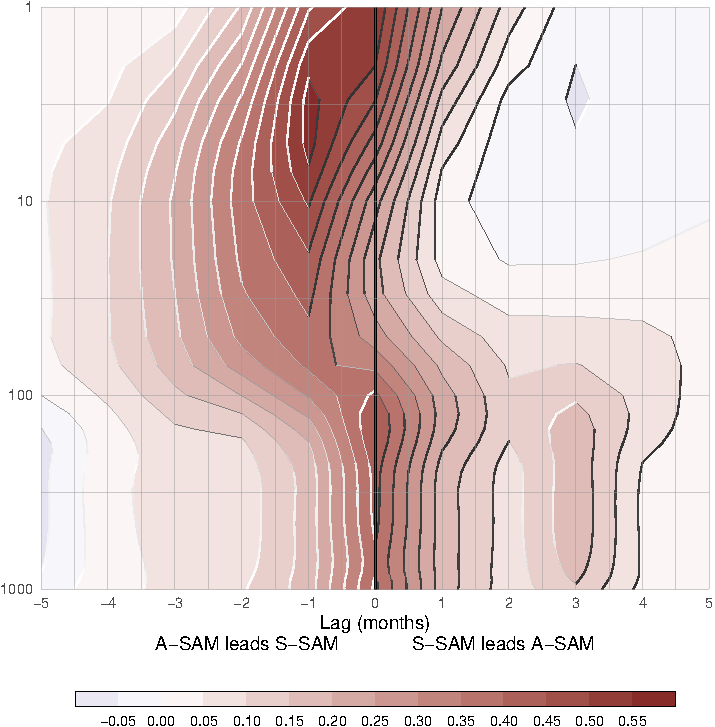
\includegraphics{A1-1} \appendcaption{A1}{Lag-correlation between Asymmetric SAM and Symmetric SAM index at each level. Negative lags imply Symmetric SAM leading Asymmetric SAM and vice versa. For the 1979 -- 2018 period.}\label{fig:A1}
\end{figure}

\begin{figure}
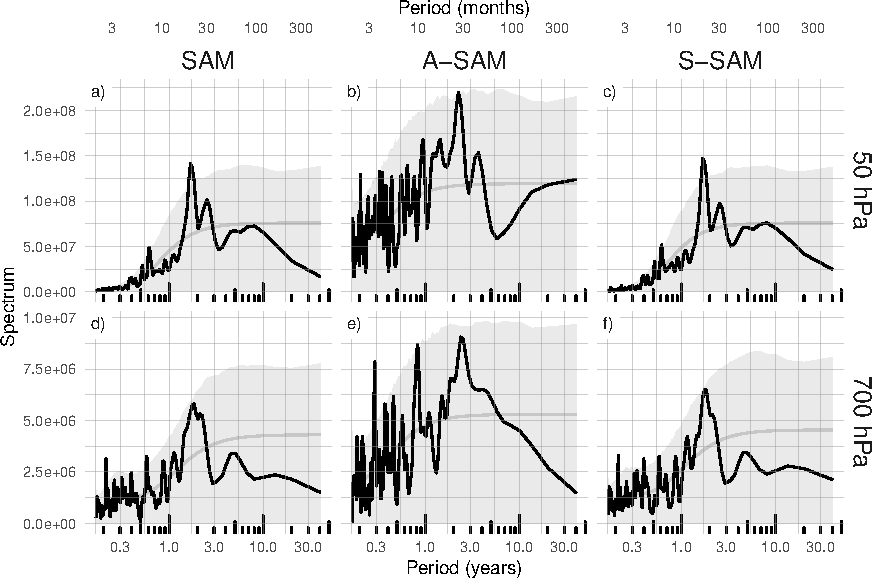
\includegraphics{A2-1} \appendcaption{A2}{Fourier spectrum of each timeseries computed as Fourier transform smoothed with modified Daniell smoothers with widths 3 and 5. The shading indicates de 95\% confidence area derived by fitting an autorregressive model and computing the spectrum for 5000 simulated samples from the fitted autoregressive model (95\% of the simulated sampels had an amplitude equal or lower). The light line indicates the theoretical expected amplitude from the autorregressive model. For the 1979 -- 2018 period.}\label{fig:A2}
\end{figure}

\begin{figure}
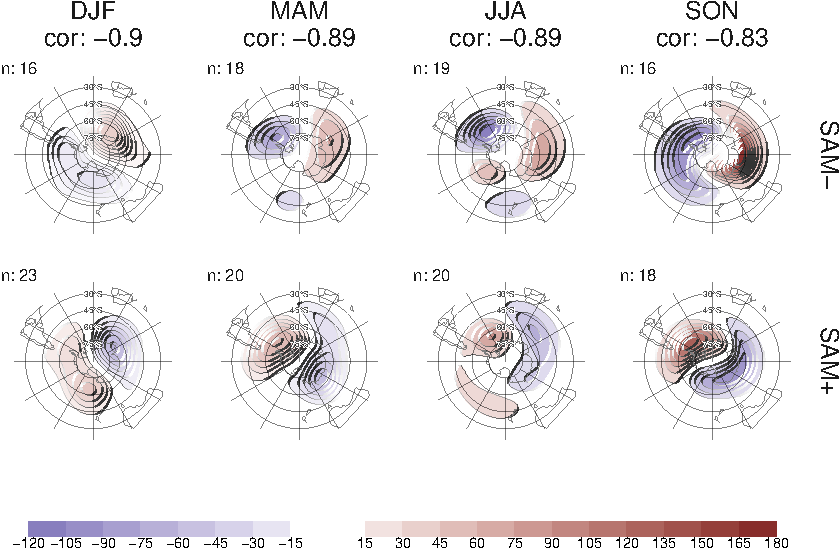
\includegraphics{A3-1} \caption[50 hPa Geopotetnial height zonal anomalies (meters) of composites of positive and negative SAM months selected using $\pm1$ standard deviation as threshhold for the 1979 -- 2018 period]{50 hPa Geopotetnial height zonal anomalies (meters) of composites of positive and negative SAM months selected using $\pm1$ standard deviation as threshhold for the 1979 -- 2018 period. Numbers in the column headers are pattern correlation between SAM+ and SAM- composites and number of monthly fields used to construct the composites.}\label{fig:A3}
\end{figure}

\begin{figure}
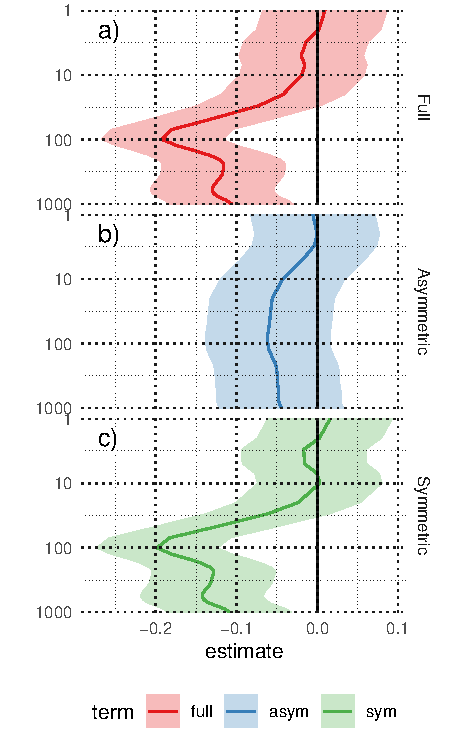
\includegraphics{A4-1} \caption[700 hPa Geopotetnial height zonal anomalies (meters) of composites of positive and negative SAM months selected using $\pm1$ standard deviation as threshhold for the 1979 -- 2018 period]{700 hPa Geopotetnial height zonal anomalies (meters) of composites of positive and negative SAM months selected using $\pm1$ standard deviation as threshhold for the 1979 -- 2018 period. Numbers in the column headers are pattern correlation between SAM+ and SAM- composites and number of monthly fields used to construct the composites.}\label{fig:A4}
\end{figure}

\begin{figure}
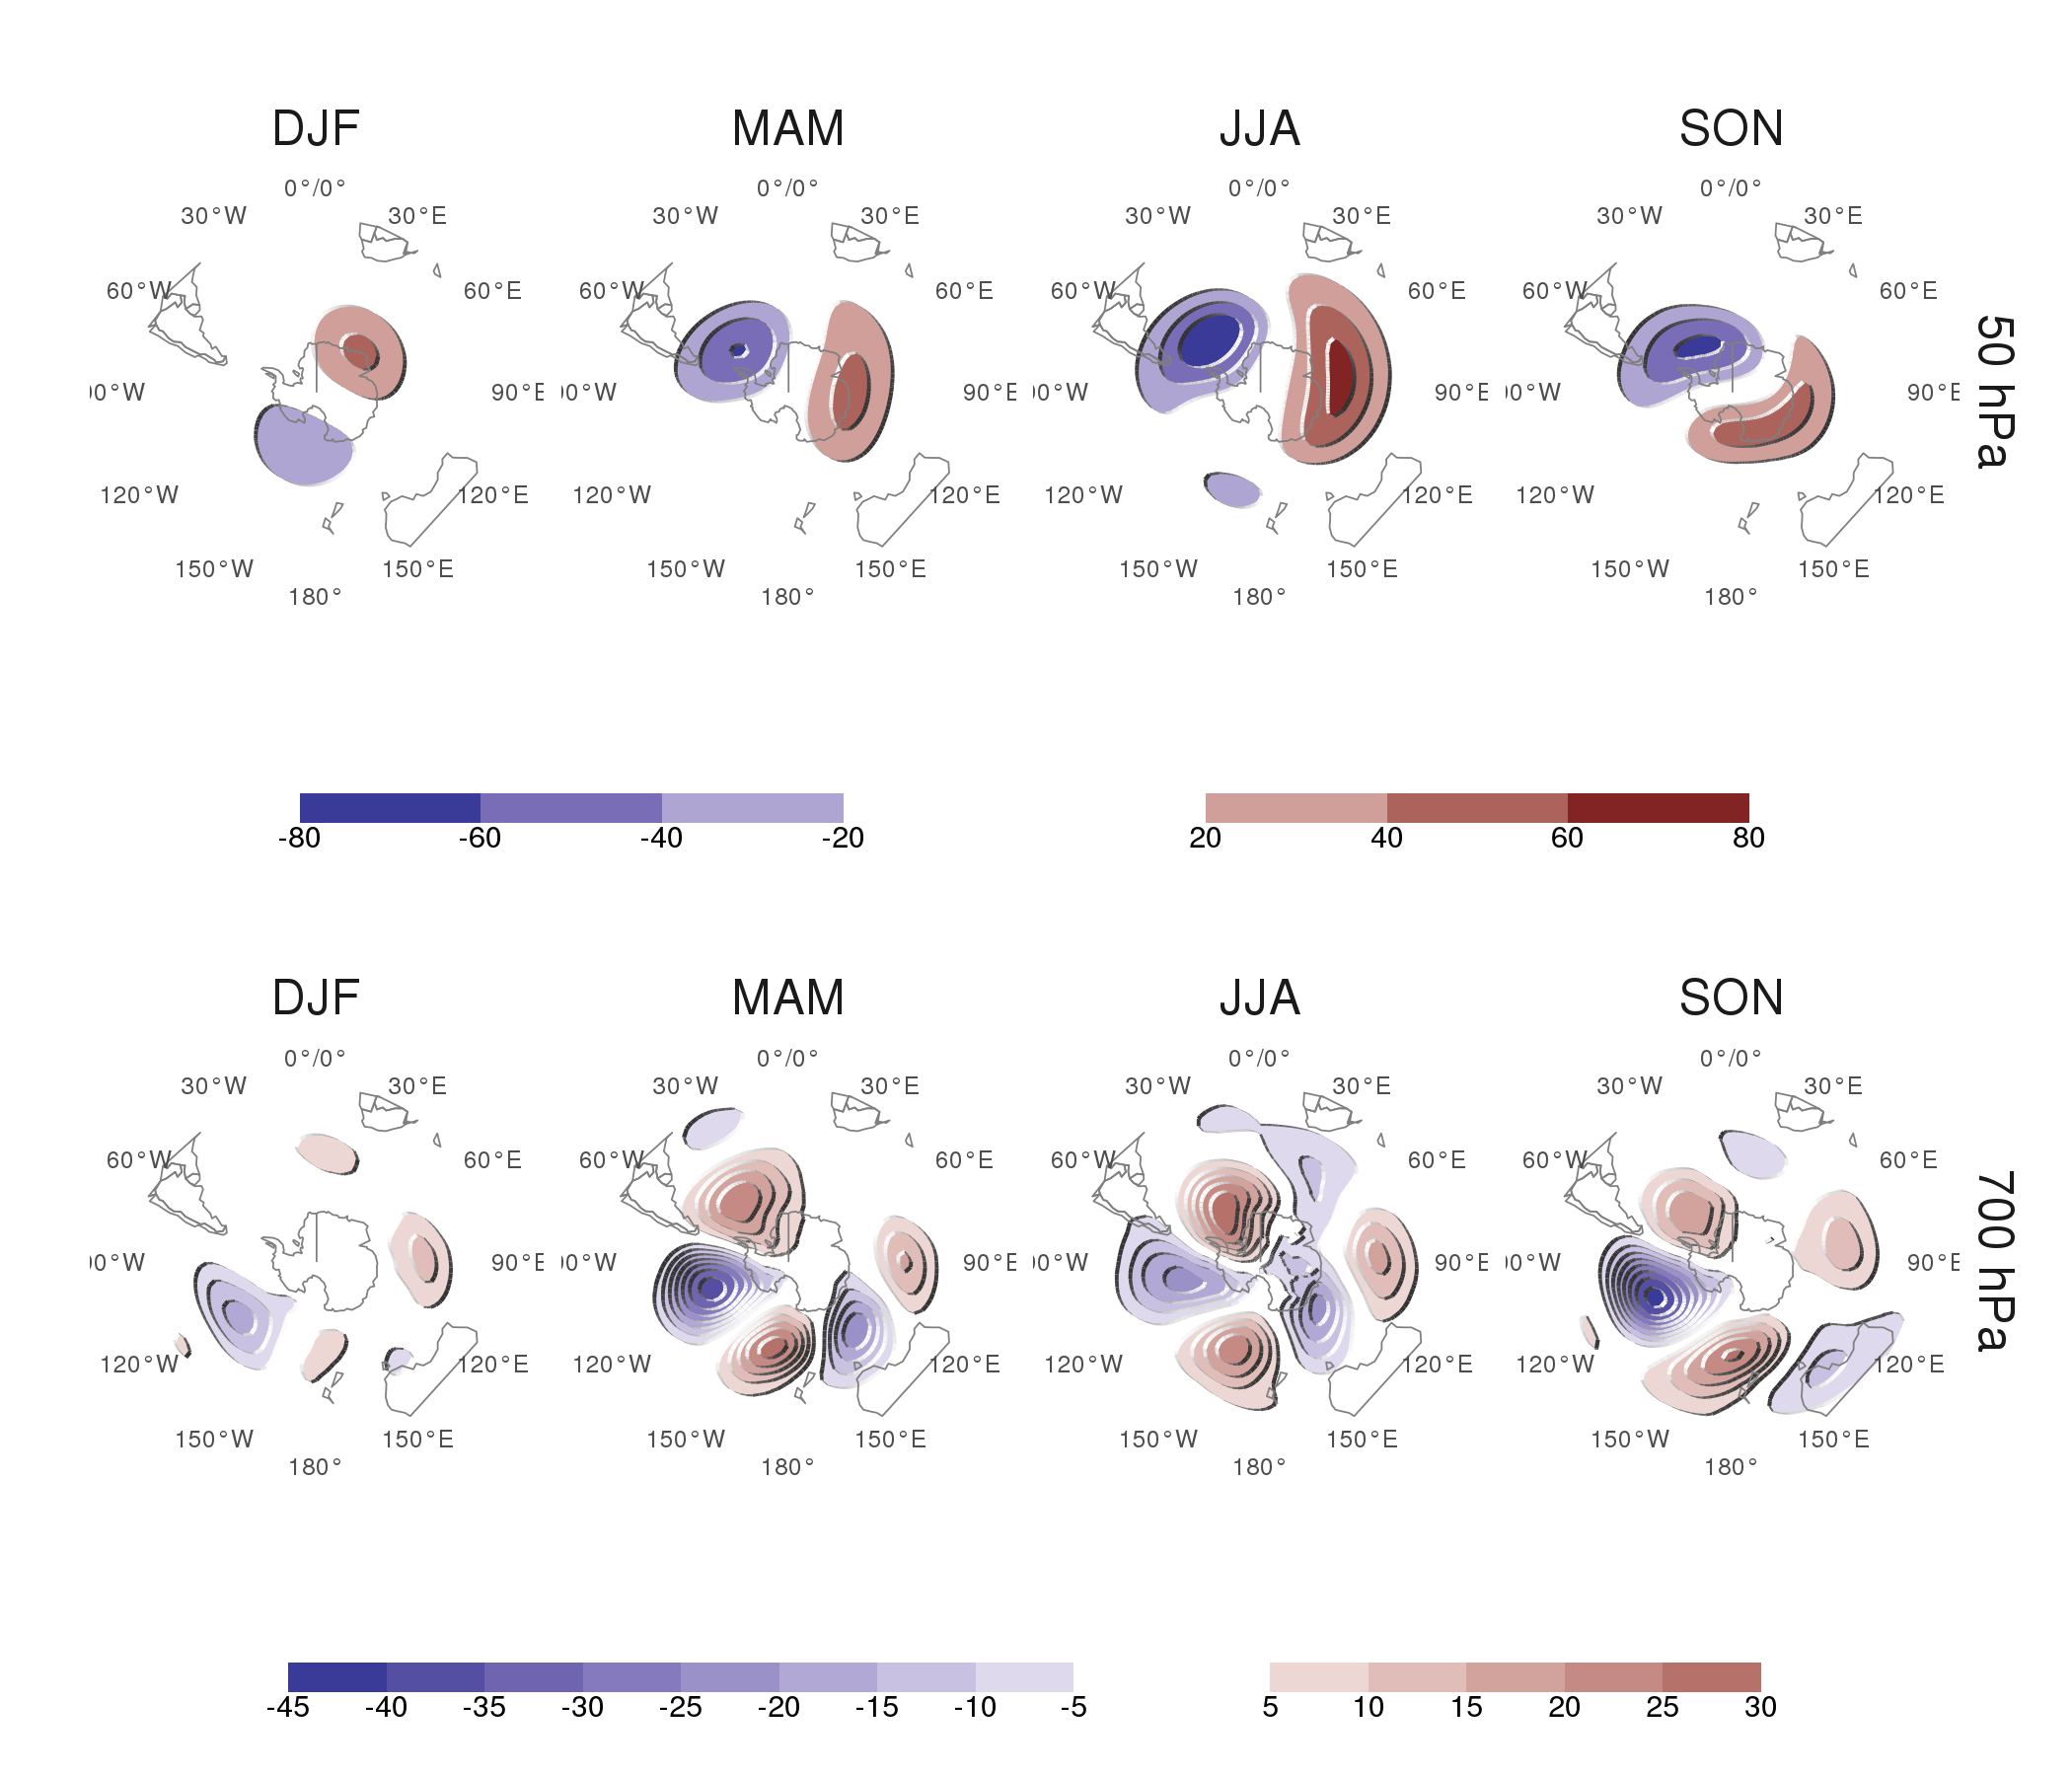
\includegraphics{A5-1} \caption[Regression coefficients of 50 hPa and 700 hPa geopotential height zonal anomalies (meters) onto the standarised timeseries of the leading EOF computed for each season independently for the 1979 -- 2018 period]{Regression coefficients of 50 hPa and 700 hPa geopotential height zonal anomalies (meters) onto the standarised timeseries of the leading EOF computed for each season independently for the 1979 -- 2018 period.}\label{fig:A5}
\end{figure}

\begin{figure}
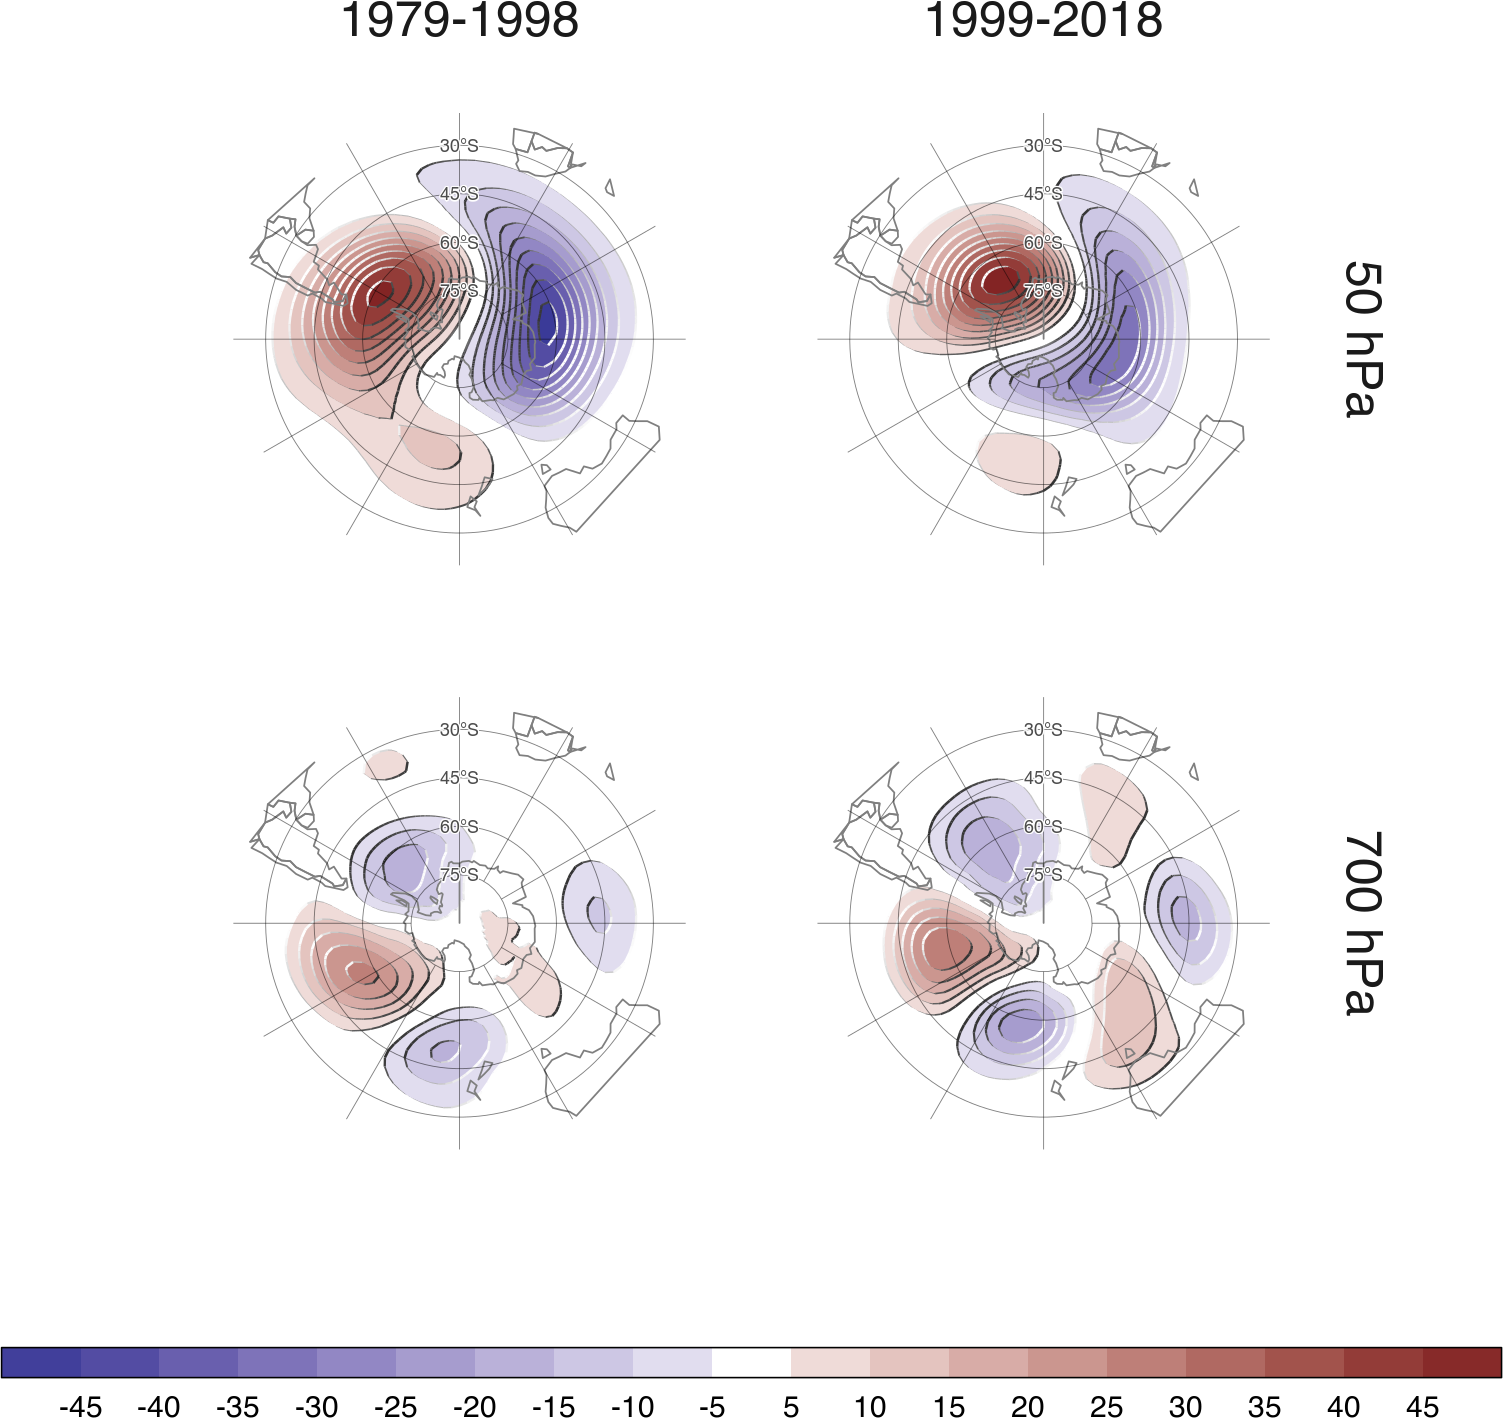
\includegraphics{A6-1} \caption[Regression of 50 hPa and 700 hPa geopotential height zonal anomalies (meters) onto the standarised timeseries of the leading EOF computed for the periods 1979 -- 1998 and 1999 -- 2018]{Regression of 50 hPa and 700 hPa geopotential height zonal anomalies (meters) onto the standarised timeseries of the leading EOF computed for the periods 1979 -- 1998 and 1999 -- 2018. Pattern correlation between both fields is 0.86 for the 50 hPa fields and 0.76 for the 700 hPa fields.}\label{fig:A6}
\end{figure}


\end{document}
